\documentclass[11pt]{article}

\usepackage[a4paper,margin=29mm]{geometry}
\usepackage[T1]{fontenc}
\usepackage{lmodern}
\usepackage{microtype}
\usepackage{amsmath,amssymb,amsthm,mathtools}
\usepackage{booktabs}
\usepackage{array}
\usepackage{float}
\usepackage{enumitem}
\usepackage{tikz}
\usetikzlibrary{positioning}
\usepackage[hidelinks]{hyperref}

\newtheorem{theorem}{Theorem}[section]
\newtheorem{proposition}[theorem]{Proposition}
\newtheorem{corollary}[theorem]{Corollary}
\newtheorem{lemma}[theorem]{Lemma}
\theoremstyle{definition}
\newtheorem{definition}[theorem]{Definition}
\newtheorem{problem}[theorem]{Problem}
\theoremstyle{remark}
\newtheorem{remark}[theorem]{Remark}

\newcommand{\PG}{\mathrm{PG}}
\newcommand{\F}{\mathbb{F}}
\newcommand{\cC}{\mathcal{C}}
\newcommand{\cU}{\mathcal{U}}
\newcommand{\A}{A_5}

\title{Deep-hole rigidity and factorization memory\\
in the Clebsch hexagon code}
\author{Tavis Rudd}
\date{Working draft --- July 2026}

\begin{document}
\maketitle

\begin{abstract}
We characterize the exceptional non-GRS $[6,3,4]_{11}$ MDS code by the
algebraic geometry of its maximum-distance syndromes.  Among all six-arcs
of $\PG(2,11)$, containment of the projective deep-hole syndrome locus in
a conic is equivalent to membership in the Clebsch class; the locus is
then the twelve rational points of a nonsingular conic and the stabilizer
is $A_5$.  A line bound, a chord-defect identity, and Dye's Brianchon
theorem prove the geometric implication.  An exact census supplies the
sharp numerical gap and the small-arc classification.

Passing to the conic code forgets the pairing of its points into secants.
We recover finite matching data by dividing differences of canonically
scaled secant products by the conic equation.  The resulting quotient
configurations have ranks $3,6,10$ in the rank-three Coxeter cases
$A_3,B_3,H_3$.  In the $B_3$ and $H_3$ cases, moment conditions recover
two complementary factorization sheets up to interchange, a signed cubic
orients them, and six explicit $H_3$ incidence profiles recover the
corresponding matching-table row.

\end{abstract}

\noindent\textbf{Keywords.} Clebsch hexagon; MDS code; deep hole; finite
projective plane; arc; conic; reflection arrangement; factorization;
orientation torsor.

\smallskip
\noindent\textbf{2020 Mathematics Subject Classification.} 51E21, 94B05,
51E22, 05B25.

\section{Introduction}
\label{sec:intro}

Let $C$ be a linear $[n,k,d]_q$ code with covering radius $\rho$ and
full-rank parity-check matrix $H$. For a received word $v$, write
$\sigma(v)=Hv^{\mathsf T}$ and
\[
 w(s)=\min\{\operatorname{wt}(e):He^{\mathsf T}=s\}.
\]
Then $d(v,C)=w(\sigma(v))$, and $v$ is a \emph{deep hole} precisely when
this minimum is $\rho$. The syndrome $s$ specifies one coset of $C$, whose
coset leaders are its weight-$w(s)$ representatives. Because
$w(\lambda s)=w(s)$ for $\lambda\ne0$, maximum-distance syndrome directions
form a projective locus
\[
 \mathcal D_{\mathrm{proj}}(C)=
 \{[s]\in\PG(n-k-1,q):w(s)=\rho\}.
\]
Thus one projective direction represents $q-1$ distinct nonzero syndrome
cosets, while each coset contains $|C|$ received words.

For an MDS code of redundancy $r=n-k$, the parity-check columns form a
projective arc in $\PG(r-1,q)$, and $w(s)$ is the least number of columns
whose span contains $[s]$. Adjoining a new column preserves the MDS property
exactly when its direction avoids every hyperplane spanned by $r-1$ existing
columns. In the redundancy-three plane case used here, this specializes to
weights one, two, or three according as the direction lies on the arc, on a
secant of the arc, or on neither; an extension point is precisely a direction
missed by every secant. We write $\cU(A)$ for this extension locus. If
$\cU(A)\ne\emptyset$, then the associated code has covering radius three
and $\cU(A)=\mathcal D_{\mathrm{proj}}(C)$. This dictionary is classical in
the theory of complete arcs and is developed for MDS codes by Davydov,
Marcugini, and Pambianco~\cite{DMP2021}; their Theorem~6.3 supplies the
leader count used in Section~\ref{sec:code}. See also
Hirschfeld~\cite{Hirschfeld1998} for the plane arc/covering-radius setting.

Henceforth \emph{uncovered locus} and $\cU(A)$ are the primary terms;
\emph{projective deep-hole syndrome locus} is their coding-theoretic synonym.
We call a line through two points of $A$ a \emph{chord}; \emph{secant}
emphasizes its incidence with $A$, while \emph{edge} refers to the
corresponding pair in the complete graph on the arc labels and \emph{join}
emphasizes construction from its two endpoints.

The three correspondences used throughout are
\[
\begin{array}{c@{\quad\longleftrightarrow\quad}l}
\text{parity-check column ray}&\text{arc point},\\
\text{non-arc point $x$ on $i$ secants}&
  \text{$i$ weight-two leaders per syndrome above $x$},\\
\text{uncovered point}&\text{projective deep-hole direction}.
\end{array}
\]

The paper studies one small exception to the GRS picture: a non-GRS
$[6,3,4]_{11}$ MDS code whose projective deep-hole locus is exactly the
$\F_{11}$-point set of a nonsingular conic. Its parity-check columns form
the \emph{Clebsch hexagon}, a six-arc in $\PG(2,11)$. Thus a natural
property of the covering-radius structure, with no assumed symmetry or
conic construction, singles out a classical configuration.

The first main theorem starts from no symmetry or conic construction.
Among all six-arcs of $\PG(2,11)$, conic containment of the projective
deep-hole syndrome locus reconstructs the Clebsch hexagon and its $A_5$
stabilizer.  A line bound, a chord-defect identity, and Dye's Brianchon
theorem give the conceptual implication; the census is needed only for the
numerical clause.  We prove quantitative gaps, reconstruct the Brianchon
geometry and an invariant support bipartition from decoder ambiguity, and
isolate $q=11$.

The second main theorem asks what remains after passing from the parent to
the full conic child.  The unmarked conic code forgets its secant matching.
The lost data reappears in the conic ideal: differences of matching-secant
products, divided by the conic equation, form a finite quotient
configuration.  Its first two moments recover the unique unordered pair of
factorization sheets, its signed cubic orients that pair, and a six-profile
double-coset compression recovers the corresponding decorated matching row
from either singleton profile.  The further identification of such a row
with a geometric Clebsch parent is not part of this theorem.  Here
\emph{orientation} means a choice in a two-element
$C_2$-torsor of sheets.  It is distinct from the intrinsic unordered
support bipartition recovered by decoder ambiguity, and has no implied
quantum-information or chiral-polytope meaning.

The reflection-arrangement model places this reconstruction in the complete
rank-three family.  For a Clebsch hexagon $K$, the chord identity gives
$|\cU(K)|=q^2-14q+45$, with off-conic excess $(q-4)(q-11)$ when
$q\equiv3\pmod4$.  The fifteen chords are reduced projectivized $H_3$
mirrors.  The six joins of a four-frame are similarly projectivized $A_3$
mirrors, and $B_3$ supplies the intermediate root-length-defect case.  At
$q=h+1=5,7,11$ the three reflection complements are full rational conics.

The configuration goes back to Clebsch~\cite[p.~336]{Clebsch1871}. Edge
constructed its finite-plane form and determined its order-$60$ stabilizer
\cite[\S\S29--32]{Edge1956}; Dye proved projective uniqueness and determined
the stabilizer over a general field~\cite[Theorems~1 and 3,
pp.~275--278]{Dye1991}; Storme and Van~Maldeghem identified the corresponding
six-arc in their finite-plane classification~\cite{SVM1995}. Deep holes of
Reed--Solomon codes have both an algorithmic history
\cite{GuruswamiVardy2005,ChengMurray2007} and a geometric classification in
the projective case~\cite{ZWK2020}. Those results concern GRS codes, whose
arcs lie on normal rational curves; the code here is not GRS.

\paragraph{Contribution and dependency boundary.}
\begin{center}
\footnotesize
\begin{tabular}{@{}>{\raggedright\arraybackslash}p{0.18\textwidth}
                    >{\raggedright\arraybackslash}p{0.36\textwidth}
                    >{\raggedright\arraybackslash}p{0.38\textwidth}@{}}
\toprule
Layer & Classical or prior input & Contribution here\\
\midrule
Clebsch geometry
& configuration, uniqueness, stabilizer, and complete exterior set
  \cite{Clebsch1871,Edge1956,Dye1991,BSW1992,SVM1995}
& symmetry-free coding criterion; low-degree rigidity, sharp gaps,
  support bipartition, decoder recovery, and field boundary\\
Six-arc census
& Sadeh's classification of six-arcs in $\PG(2,11)$
  \cite{SadehThesis1984}
& independent frame-normalized replay; no priority claim for the census
  or extension counts\\
Reflection arrangement
& icosahedral realization and $H_3$ ledger
  \cite[\S\S19--20]{Edge1956}\cite{Calvo2024}; finite-field method
  \cite{Athanasiadis1996}; arrangement enumerators
  \cite[Prop.~3.11, Thms.~5.3, 5.7, Ex.~5.10]{JurriusPellikaan2015}
& explicit reduced-$H_3$--code bridge, decoder specialization, and common
  $A_3/B_3/H_3$ conic phase\\
Matching data
& one-factorizations, $5,14,22$ marker fibres, matching designs, and
  coarse Hadamard orbitals
& conic-ideal quotient, balanced recovery, cubic orientation, depth
  compression, and matching-row recovery\\
\bottomrule
\end{tabular}
\end{center}
The companion arcs paper also records
Proposition~\ref{prop:deep-holes-conic} with a kernel-checked theorem
\cite[Prop.~8.2]{ArcsCompleteOutsideConic}; we reprove it here, and no
result depends on that paper.

\section{A guided tour of forgetting and memory}
\label{sec:tour}

The reconstruction problem begins with a tension.  The projective
deep-hole locus of the Clebsch code is exceptionally rigid: its containment
in a conic determines the Clebsch class.  The conic itself is familiar and
forgetful: its twelve rational points support the extended Reed--Solomon
code, with no preferred pairing, parent, or orientation.  Figure
\ref{fig:reconstruction-arc} records how the missing information returns.

\begin{figure}[H]
\centering
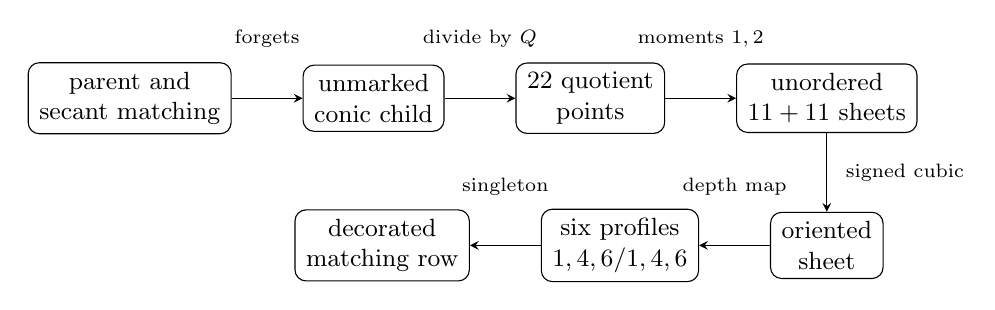
\begin{tikzpicture}[
  every node/.style={align=center,font=\small},
  box/.style={draw,rounded corners,minimum height=8mm,inner xsep=4pt},
  edge label/.style={font=\scriptsize,fill=white,inner sep=1pt},
  >=stealth]
\node[box] (p) {parent and\\secant matching};
\node[box,right=9mm of p] (c) {unmarked\\conic child};
\node[box,right=9mm of c] (q) {$22$ quotient\\points};
\node[box,right=9mm of q] (s) {unordered\\$11+11$ sheets};
\node[box,below=10mm of s] (o) {oriented\\sheet};
\node[box,left=9mm of o] (d) {six profiles\\$1,4,6/1,4,6$};
\node[box,left=9mm of d] (r) {decorated\\matching row};
\draw[->] (p) -- node[edge label,above=6mm]{forgets} (c);
\draw[->] (c) -- node[edge label,above=6mm]{divide by $Q$} (q);
\draw[->] (q) -- node[edge label,above=6mm]{moments $1,2$} (s);
\draw[->] (s) -- node[edge label,right=2mm]{signed cubic} (o);
\draw[->] (o) -- node[edge label,above=6mm]{depth map} (d);
\draw[->] (d) -- node[edge label,above=6mm]{singleton} (r);
\end{tikzpicture}
\caption{The matching-data recovery arc.  The arrows are respectively a forgetting
map, an ideal-quotient construction, intrinsic recovery of an unordered
partition, a torsor orientation, a profile map, and decorated table-row
recovery; they are not all linear quotients.}
\label{fig:reconstruction-arc}
\end{figure}

For a perfect matching $M$ of the conic points, let $P_M$ be the product of
its secant equations under the canonical bracket scaling of
Section~\ref{sec:factorization}.  All $P_M$ have the same restriction to the
conic, so $(P_M-P_N)/Q$ is a polynomial.  The Coxeter-selected matchings
give the finite quotient configurations used below.

\begin{theorem}[Rigidity and the rank-three conic phase]
\label{thm:headline-rigidity-phase}
The following statements hold.
\begin{enumerate}[label=\textup{(A\arabic*)},leftmargin=*]
\item Among six-arcs of $\PG(2,11)$, conic containment of the full
projective deep-hole locus characterizes the Clebsch class and recovers its
$A_5$ stabilizer.
\item Let $T\in\{A_3,B_3,H_3\}$ have Coxeter number $h$, and reduce its
displayed standard arrangement over a lattice-good finite field $\F_q$ in
the determinant sense of Proposition~\ref{prop:lattice-good}.  Thus the
characteristic is odd, with a chosen image of $\tau$ for $H_3$.  Whenever
the complement is nonempty, its projective evaluation code has parameters
\[
 \bigl[(q-h/2)(q-h+1),\,3,\,
       (q-h/2-1)(q-h+1)\bigr]_q;
\]
a nonmirror line meets the complement in at most $q-h+1$ points.
\item In the three specializations $q=h+1$, namely
$(A_3,5),(B_3,7),(H_3,11)$, the complement is the full rational conic and
its projective-system code is extended GRS.
\item In those three specializations, the square of a Coxeter element
generates the split maximal torus in $\mathrm{PSL}_2(q)$, and its two
moving point-orbits are the two Legendre cosets.
\end{enumerate}
\end{theorem}
\noindent\emph{Proof mode: mixed.}  The rigidity implication is a human
proof with one cited classical theorem; the numerical gap is an exhaustive
exact enumeration.
The rank-three clauses combine the human specialization and distance
proofs of Section~\ref{sec:coxeter-number-phase}, Lean-checked algebra,
exhaustive exact ledgers, and cited classical group identifications.

\begin{theorem}[Factorization recovery]
\label{thm:headline-factorization}
\begin{enumerate}[label=\textup{(F\arabic*)},leftmargin=*]
\item All canonically scaled matching-secant products have equal
restriction to the conic; every four-endpoint switch difference is
divisible by $Q$.  The $A_3,B_3,H_3$ quotient configurations have linear
ranks $3,6,10$, respectively.
\item In the $B_3$ and $H_3$ configurations, the two Coxeter
factorization sheets are, up to interchange, the unique complementary
halves having equal first and second tensor moments.
\item With opposite signs on the two sheets, every even signed profile
moment vanishes, and the primitive weighted barycentre relation
$v_1+4v_4+6v_6=0$ kills degree one.  Within the signed tensor-moment
family and its linear functionals, degree three is the first surviving
degree; its nonzero tensor transforms by the outer character.
\item For $G=\mathrm{PGL}_2(11)$, $H=A_5$, and the common
$K=A_4$, the space $K\backslash G/H$ has six labels in two triples of
sizes $1,4,6$, with profiles
$v_1,v_4,v_6,-v_1,-v_4,-v_6$.  The profile map has rank two and
four-dimensional linear kernel but separates the six labels.  Its
singleton profiles recover the unordered $H_3$ matching pair, and a
choice of singleton recovers the corresponding row of the frozen matching
table.  No geometric-parent identification is asserted.
\end{enumerate}
\end{theorem}
\noindent\emph{Proof mode: mixed.}  The quotient and moment implications
are proved in the text and Lean; the three finite configurations, their
ranks, and the six profile rows are checked by exhaustive exact replay.

The sequence $22\to6\to2\to1$ is an information ledger, not a chain of
faithful linear images.  In particular, the two-dimensional profile plane
is not the two-element sheet set.  Sections
\ref{sec:factorization}--\ref{sec:survival} prove the new arrows after the
rigidity and Coxeter inputs have been established.

\paragraph{How the proofs divide.}
The headline arguments isolate mechanisms: the Pl\"ucker relation remembers
factorization modulo the conic ideal; an annihilator line forces the
balanced sheets; antipodality and the primitive $1:4:6$ relation force
cubic-first orientation; projective-cover structure explains the depth
plane; and determinant-sign descent identifies the surviving bit.  Exact
finite computations verify the frozen orbit, rank, and normalizer
hypotheses used by these arguments.  They are supporting certificates; the
preceding structures explain the headline theorems.

\paragraph{Proof modes for the headline results.}
The rigidity implication in (A1) is a human proof using Dye's classical
Brianchon theorem; only its numerical gap uses the exhaustive
$1548$-representative census.  Clauses (A2)--(A4) are mixed: the uniform
algebra is proved in the text and Lean, while the coordinate-to-Coxeter
identifications are cited or verified by exhaustive exact replay.  Clause (F1) combines
the displayed Pl\"ucker proof with exact rank calculations; (F2)--(F4)
combine the stated moment and double-coset arguments with exhaustive
finite tables.  The arithmetic-gluing, holonomy, and determinant-sign
results below are also marked as mixed at their statements: their
structural implications are proved in the text, while their frozen finite
hypotheses are verified by exhaustive exact replay.  Section~\ref{sec:verification} gives
the terminal- and artifact-level boundaries.

\paragraph{Independence and extension.}
The unlabelled child admits no equivariant selector of a matching row,
whereas a marked matching supplies the one bit needed to choose between
the two sheets.  Thus the obstruction is the absence of an equivariant
section, and the marked extension resolves exactly that two-valued
ambiguity.

\section{The Clebsch hexagon}
\label{sec:hexagon}

Fix the nonsingular conic
\[
 \cC:\ XZ=Y^2
\]
in $\PG(2,11)$, with its $12$ points identified with $\PG(1,11)=\F_{11}\cup\{\infty\}$
in the usual way. The stabilizer of $\cC$ in $\mathrm{PGL}(3,11)$ is
$\mathrm{PGL}_2(11)$, acting on $\cC$ as it acts on the projective line.

A convenient representative is
\[
 A=\{(1,10,0),\,(1,9,1),\,(1,4,7),\,(1,8,5),\,(0,1,4),\,(1,1,7)\}.
\]
It is a six-arc disjoint from $\cC$; its fifteen joins also avoid $\cC$.
The following invariant construction explains its symmetry.

\begin{definition}[Clebsch hexagon]
\label{def:hexagon}
Let $\A\subset\mathrm{PGL}_2(11)$ be an icosahedral subgroup. The
six Sylow $5$-subgroups of $\A$ each fix two points of $\cC$. The
\emph{Clebsch hexagon} is the set of poles of the six chords joining these
fixed pairs.
\end{definition}

For a nonsingular conic over an odd field, an \emph{external point} lies on
two tangents and an \emph{internal point} on none; an external, or
\emph{passant}, line is disjoint from the conic.
Edge's six vertices are external, their fifteen joins are external, and
those joins concur three at a time at ten internal Brianchon
points~\cite[\S\S29--32]{Edge1956}. Thus the hexagon is a complete exterior
set in the terminology of Blokhuis, Seress, and Wilbrink
\cite[pp.~143,146]{BSW1992}. Their $q=11$ list also contains a Pasch
configuration, but its four collinear triples prevent it from defining an
MDS code. Thus exteriority alone gives only
$\cC(\F_{11})\subseteq\cU(A)$; the arc hypothesis selects the Clebsch
branch, and Proposition~\ref{prop:deep-holes-conic} proves equality.

This is the arc $K_2$ of Storme and Van~Maldeghem
\cite[Props.~11--12]{SVM1995} and Dye's synthetic hexagon when $5$ is a
square in the base field~\cite[Theorem~1]{Dye1991}. Dye proves uniqueness,
stabilizer $A_5$, and the unique associated polarity; in the displayed
coordinates its conic is $\cC$. His calculation also shows that the six
vertices lie on no conic in characteristic $11$
\cite[Theorem~2, pp.~277--278; p.~281]{Dye1991}. Storme and Van~Maldeghem
record that the arc is incomplete at $q=11$~\cite[Prop.~13]{SVM1995}, so the
associated redundancy-three code has covering radius three.

\section{The code and its projective syndrome locus}
\label{sec:code}

Take the parity-check matrix
\[
 H=
 \begin{pmatrix}
  1&1&1&1&0&1\\
 10&9&4&8&1&1\\
  0&1&7&5&4&7
 \end{pmatrix},
\]
whose columns are the six displayed points of $A$, and let
\[
 C=\{c\in\F_{11}^6:Hc^{\mathsf T}=0\}
\]
be the resulting $[6,3,4]_{11}$ MDS code. Since the six columns of $H$ do
not lie on any conic (their evaluation matrix against the six quadratic
monomials $X^2,XY,XZ,Y^2,YZ,Z^2$ is nonsingular), $C$ is not monomially
equivalent to a GRS code: the dual of a GRS code is GRS, and the parity-check
column system of a length-six, dimension-three GRS code lies on a normal
rational curve, here a conic, in the classical
normal-rational-curve/GRS dictionary~\cite{StormeThas1991}.

The arc--coset dictionary from the introduction applies without a GRS
hypothesis~\cite[Def.~6.1, Thm.~6.3]{DMP2021}. Each uncovered direction
$x$ lifts to $q-1$ weight-three cosets, and each has
$\binom{6}{3}=20$ minimum-weight leaders. Geometrically, the same condition says
that adjoining $x$ as a seventh column preserves the MDS property.

For example, $s=(1,0,0)$ lies on $\cC$ and is therefore uncovered.
The error
\[
 e=(7,4,1,0,0,0)
\]
satisfies $He^{\mathsf T}=s$.  No error of weight one or two has syndrome
$s$, while the twenty triples of coordinate positions each support one
weight-three leader.  Thus this single syndrome exhibits the complete
dictionary: its projective direction is a conic point, its coset has
distance three, and its nearest-codeword ambiguity has size twenty.

The stabilizer already forces the small point sets that will occur.

\begin{proposition}[The $A_5$ point orbits]
\label{prop:a5-point-orbits}
Let $G=\operatorname{Stab}(A)\cong A_5$. Its orbits on $\PG(2,11)$ have
lengths
\[
 6,\ 10,\ 12,\ 15,\ 30,\ 30,\ 30.
\]
The first four are respectively $A$, the ten Brianchon points,
$\cC(\F_{11})$, and the fifteen vertices of the five self-polar triangles.
In particular, $\cC(\F_{11})$ is the unique twelve-point $G$-orbit.
\end{proposition}

\begin{proof}
Dye's polarity and stabilizer theorems identify $G$ with the ternary
icosahedral representation preserving $\cC$, and his Corollary~1 makes it
transitive on the six vertices, ten Brianchon points, and fifteen triangle
vertices~\cite[Theorems~2--3 and Corollary~1, pp.~276--279]{Dye1991}.
We derive the orbit sizes without using the finite enumeration.

The argument first determines the points with each possible nontrivial
stabilizer, then applies orbit--stabilizer to recover the orbit lengths.

Since $11\nmid60$, the representation is semisimple, and the ternary
icosahedral representation is irreducible; hence $G$ fixes no projective
point. The ordinary
three-dimensional icosahedral character, reduced in $\F_{11}$, shows that
an involution, an element of order three, and an element of order five fix
respectively $13$, $1$, and $3$ projective points. Indeed, an involution
has a one-dimensional eigenspace and a two-dimensional eigenspace; the
nontrivial order-three eigenvalues are not in $\F_{11}$; and the three
order-five eigenvalues are distinct because $5\mid10$. Restricting the same
representation to the standard subgroups of $A_5$ gives the following
common-fixed-point ledger; the standard subgroup classification of $A_5$
shows that these are all possible nontrivial proper point stabilizers. Here
$D_5$ has order ten, and the last row counts points whose stabilizer is
exactly the displayed subgroup type.
For the noncyclic entries, determine the common projective eigenlines of
standard generators: a $D_5$ normalizer retains one of the three $C_5$
eigenlines, an $S_3$ normalizer retains the unique $C_3$ eigenline, a $V_4$
has three
simultaneous eigenlines, and its overgroup $A_4$ permutes those three and
fixes none. This gives the second row.
\[
\begin{array}{c|rrrrrr}
H&A_4&D_5&S_3&C_5&V_4&C_3\\ \hline
\text{number of conjugate subgroups}&5&6&10&6&5&10\\
\text{fixed points for one }H&0&1&1&3&3&1\\
\text{points with stabilizer conjugate to }H&0&6&10&12&15&0
\end{array}
\]
By orbit--stabilizer, the third row already gives the orbits of lengths
$6$, $10$, $12$, and $15$; only points with exact stabilizer $C_2$ remain.
To spell out the subtraction in the last row: the normalizer $D_5$ fixes
one of the three $C_5$ eigenlines and interchanges the other two, giving
$6$ points with stabilizer $D_5$ and $12$ with stabilizer $C_5$; the unique
$C_3$-fixed line is already fixed by its $S_3$ normalizer; and $A_4$ cycles
the three $V_4$ eigenlines, leaving all fifteen with exact stabilizer $V_4$.

It remains to account for exact $C_2$ stabilizers. Each involution lies in
two $D_5$ subgroups, two $S_3$ subgroups, and one $V_4$. Of its thirteen
fixed points, these contribute respectively $2$, $2$, and $3$ points from
the preceding rows. The remaining six points have exact stabilizer $C_2$.
There are fifteen involutions, so this gives $90$ points, necessarily three
orbits of length $60/2=30$. The total
$6+10+12+15+90=133$ exhausts the plane. Dye's Theorem~6(v), specialized at
$q=11\equiv1\pmod{10}$, identifies the twelve-point $C_5$-stabilizer orbit
with $\cC(\F_{11})$~\cite[pp.~281--282; \S3.1, p.~284]{Dye1991}; the other
three identifications are the transitive sets cited above.
\end{proof}

\begin{proposition}[The uncovered locus is the conic]
\label{prop:deep-holes-conic}
The covering radius of $C$ is three, and
\[
 \cU(A)=\mathcal D_{\mathrm{proj}}(C)=\cC(\F_{11}).
\]
\end{proposition}

\begin{proof}
The set $\cU(A)$ is $G$-invariant. Dye's Clebsch classification gives
exactly ten Brianchon points. The relevant double count is short.
The fifteen edges contribute $150$ off-arc incidences. The $45$ pairs of
disjoint edges meet once, so if $n_i$ counts off-arc points lying on exactly
$i$ edges, then a point on three edges accounts for
$\binom{3}{2}=3$ such pairs and
\[
 n_1+2n_2+3n_3=150,
 \qquad n_2+3n_3=45,
 \qquad n_3=10.
\]
Thus the edges cover $n_1+n_2+n_3=115$ of the $127$ off-arc points, leaving
$|\cU(A)|=12$. This is the $q=11$ specialization of the chord-defect
identity in Lemma~\ref{lem:chord-defect}.
By definition $\cU(A)$ is disjoint from the unique six-point orbit $A$.
The orbit lengths in Proposition~\ref{prop:a5-point-orbits} therefore force
this invariant twelve-set to be the unique twelve-point orbit
$\cC(\F_{11})$. By the dictionary above this is exactly the projective
deep-hole syndrome locus, and its nonemptiness gives covering radius three
rather than two. Dye's edge criterion and the complete-exterior-set
description of Blokhuis--Seress--Wilbrink independently supply the classical
inclusion $\cC(\F_{11})\subseteq\cU(A)$
\cite[discussion preceding Theorem~6, p.~281]{Dye1991}; see also
\cite[pp.~143, 146]{BSW1992}.
\end{proof}

\begin{corollary}[Directions, cosets, leaders, and received words]
\label{cor:named-variety}
$\cU(A)$ has $12$ directions, exactly the points of $\cC$. Above them lie
$12(11-1)=120$ nonzero maximum-distance
syndromes, hence $120$ deep-hole cosets. Each such coset has
$\binom{6}{3}=20$ minimum-weight leaders, for $2400$ leaders in all, and
contains $|C|=11^3=1331$ received words. Consequently $C$ has
$120\cdot1331=159720$ received-word deep holes.
\end{corollary}

\begin{proof}
Immediate from Proposition~\ref{prop:deep-holes-conic}, the leader-count
clause of the DMP dictionary, and the fact that the fiber of
$\F_{11}^3\setminus\{0\}\to\PG(2,11)$ over each direction consists of ten
nonzero syndromes, hence ten distinct cosets. Every coset has $|C|$ words.
\end{proof}

\subsection{Automorphisms and deep-hole orbits}
\label{sec:automorphisms}

The projective stabilizer of the six column rays is $A_5$ of order $60$,
acting faithfully and $2$-transitively on the coordinate supports. It is
the support-permutation quotient of the monomial automorphism group:
\[
 1\longrightarrow\F_{11}^{\times}\longrightarrow
 \operatorname{MAut}(C)\longrightarrow A_5\longrightarrow1.
\]
The kernel consists of the ten global coordinate scalars. The sequence
splits. Since $\gcd(3,10)=1$, each projective class has a unique
determinant-one representative; their monomial lifts give an $A_5$
complement. Hence
\[
 \operatorname{MAut}(C)\cong C_{10}\times A_5
\]
has order $600$. For the displayed column representatives, the subgroup of
pure coordinate permutations is trivial.

\begin{proposition}[One orbit on received-word deep holes]
\label{prop:deep-hole-orbit}
The monomial automorphism group of $C$ is transitive on the $120$ deep-hole
cosets. Let $\Gamma$ be the group generated by these automorphisms and by
translations $v\mapsto v+c$ for $c\in C$. Then
\[
 |\Gamma|=|C|\,|\operatorname{MAut}(C)|=1331\cdot600=798600,
\]
and $\Gamma$ is transitive on all $159720$ received-word deep holes. The
stabilizer of each such word is cyclic of order five.
\end{proposition}

\begin{proof}
The projective stabilizer $A_5$ is transitive on the twelve points of
$\cC$. Indeed, its six Sylow $5$-subgroups form one conjugacy class, each
fixes the two endpoints of one of the six fixed-point chords, and the involution in
its dihedral normalizer interchanges those endpoints. These twelve endpoints
exhaust $\cC(\F_{11})$. Every such
projectivity lifts to a monomial automorphism of the parity-check columns,
so the monomial group is transitive on the twelve syndrome rays above
$\cC$. Its central scalar subgroup $\F_{11}^{\times}$ acts transitively on
the ten nonzero vectors of each ray. Hence the monomial group is transitive
on all $12\cdot10=120$ maximum-distance syndromes and therefore on the
corresponding cosets. Given deep
holes $v$ and $w$, choose $m\in\operatorname{MAut}(C)$ with
$\sigma(mv)=\sigma(w)$. Then $c=w-mv$ has zero syndrome, so $c\in C$, and
the codeword translation by $c$ sends $mv$ to $w$. Both kinds of generator
are Hamming isometries preserving $C$. The monomial group normalizes the
translation subgroup, since $m\,t_c\,m^{-1}=t_{m(c)}$ with $m(c)\in C$.
Thus $\Gamma=C\rtimes\operatorname{MAut}(C)$; the two subgroups have trivial
intersection and the displayed product order follows. Orbit--stabilizer now gives stabilizer order
$798600/159720=5$, and every group of prime order is cyclic.
\end{proof}

\subsection{Decoding consequences}

The coset-leader-weight distribution of $C$ is $(1,60,1150,120)$
(cosets of weight $0,1,2,3$, summing to $11^3=1331$); the last entry counts
deep-hole cosets, not received words. Its codeword weight enumerator is
$(1,0,0,0,150,420,760)$, forced by the MDS parameters.

The special geometry also makes distance diagnosis and nearest-word structure
unusually explicit.  Write a syndrome as $s=(s_0,s_1,s_2)$ and put
$Q(s)=s_0s_2-s_1^2$.
For a point $x\notin A$, its \emph{secant index} is the number of chords of
$A$ through $x$; by the dictionary above, this is the number of
weight-two leaders for each nonzero syndrome on the ray $x$.

\begin{proposition}[Complete syndrome oracle and ambiguity enumerator]
\label{prop:decoding-oracle}
For $v\in\F_{11}^6$ with syndrome $s=Hv^{\mathsf T}$,
\[
 d(v,C)=
 \begin{cases}
 0,&s=0,\\
 1,&[s]\in A,\\
 3,&s\ne0\text{ and }Q(s)=0,\\
 2,&\text{otherwise}.
 \end{cases}
\]
Among the $1330$ nonzero cosets, the numbers having respectively one, two,
three, and twenty nearest codewords are
\[
 960,\qquad150,\qquad100,\qquad120.
\]
For a distance-two syndrome the number of nearest codewords is the secant
index of its direction. Every distance-three syndrome has exactly one
leader on each of the
twenty three-element coordinate supports.
\end{proposition}

\begin{proof}
The DMP dictionary identifies weight-one directions with the six columns,
weight at most two with the secant union, and weight three with its
complement.  Proposition~\ref{prop:deep-holes-conic} identifies the last
set with $Q=0$, proving the oracle.  In the notation of its proof, the
chord-intersection equations give
$(n_0,n_1,n_2,n_3)=(12,90,15,10)$, later recognized as the $H_3$
strata in Section~\ref{sec:reflection-exceptions}, where $n_i$ counts
projective directions of secant index $i$ and $n_0$ is the uncovered locus.
Every direction has
ten nonzero affine syndromes.  Thus the distance-two cosets contribute
$900$ cases of multiplicity one, $150$ of multiplicity two, and $100$ of
multiplicity three; the sixty weight-one cosets add sixty more cases of
multiplicity one.  Leaders are in bijection with nearest codewords by
translation within the coset.  Finally, the three columns on any support are independent.
For an uncovered syndrome their unique coefficients are all nonzero, since
a zero coefficient would put the syndrome on a secant.  Hence all twenty
supports, and no others, give its weight-three leaders.
\end{proof}

\subsection{Self-polar structure}
\label{sec:structural}

Edge's finite-plane construction
\cite[\S\S30.2--31]{Edge1956} and Dye's general-field synthetic theory
\cite[Theorem~2, pp.~277--278]{Dye1991} exhibit five triangles on the six
vertices, self-polar for $\cC$. Their vertex-pair matchings partition the
fifteen pairs into a \emph{synthematic total}, that is, a partition of the
edges of $K_6$ into five perfect matchings. Section~\ref{sec:chirality}
turns its ten pairs of matchings into the Brianchon--support dictionary.

\section{The rigidity theorem}
\label{sec:rigidity}

Proposition~\ref{prop:deep-holes-conic} concerns one known arc. The following theorem is the
paper's main claim: among \emph{all} six-arcs of $\PG(2,11)$, the property
``the uncovered locus lies on a conic'' picks out the
Clebsch hexagon uniquely, and does so in a way that recovers its projective
stabilizer from the coding condition rather than assuming it.

\begin{remark}[Two conditions, one word apart]
\label{rem:not-the-usual-condition}
The condition studied here is that $\cU(A)$ --- the projective uncovered,
or projective deep-hole syndrome, locus --- lies on a conic. It is
\emph{not} the familiar condition that the arc $A$ itself
lies on a conic, which is the standing hypothesis throughout the arc
literature and which the Clebsch hexagon famously fails. The two are
logically unrelated: they constrain different point sets, and the arcs
satisfying them are disjoint. Indeed every six-arc lying \emph{on} a conic in
$\PG(2,11)$ has $|\cU(A)|\in\{18,19,20,22\}$, so clause~(iii) of
Theorem~\ref{thm:rigidity} below excludes all of them. This four-value assertion is
the conic-inscribed subcensus of the independent rigidity replay listed in
Table~\ref{tab:replays}.
\end{remark}

We first isolate the geometric input that removes degenerate conics from the
computer-assisted part of the argument.

The external-line case is a six-point instance of the nonexistence in odd
order of nontrivial \emph{hyperfocused arcs}, whose secants determine only
$k-1$ points on an external line
\cite{BicharaKorchmaros1982,DrakeKeating2004,NgWild2001}. We give a direct
proof because the three possible line positions are then handled together.

\begin{lemma}[Six-arc line bound]
\label{lem:six-arc-line-bound}
Let $A$ be a six-arc in $\PG(2,q)$, where $q$ is odd. Every line contains at
most $q-5$ points of $\cU(A)$.
\end{lemma}

\begin{proof}
A chord contains no point of $\cU(A)$. If a non-chord line $\ell$ contains
one vertex, the ten chords on the other five vertices meet $\ell$ in at
least five distinct points. Indeed, two of those chords sharing an endpoint
meet only at that endpoint, which lies off $\ell$; their intersections with
$\ell$ therefore give a proper edge-colouring of $K_5$, whose chromatic
index is five. Together with the vertex, at least six of the $q+1$ points
of $\ell$ are therefore outside $\cU(A)$.

It remains to consider $\ell\cap A=\varnothing$. The fifteen chords meet
$\ell$ in covered points, and at most three chords pass through any one of
them: chords sharing an endpoint meet only at that arc vertex, not on
$\ell$, so all chords through one point of $\ell$ have disjoint endpoint
pairs. Hence there are at least five covered points. Equality would give a
proper five-edge-colouring of
$K_6$, necessarily a one-factorization. After relabelling, three factors
are
\[
  01|23|45,\qquad 02|14|35,\qquad 03|15|24.
\]
Send $\ell$ to infinity and normalize the first two directions to horizontal
and vertical. Put $p_0=(0,0)$, $p_1=(x,0)$ and $p_2=(0,y)$, where
$xy\ne0$. Writing $p_3=(a,y)$, the first two factors force
$p_4=(x,b)$ and $p_5=(a,b)$. Parallelism of $03$ with $15$ and with $24$
gives two determinant equations whose difference is $2xy=0$, impossible
for odd $q$. Thus a disjoint line has at least six covered points, and in
all cases at most $(q+1)-6=q-5$ points of $\cU(A)$ remain.
\end{proof}

\begin{theorem}[Rigidity theorem]
\label{thm:rigidity}
For a six-arc $A\subset\PG(2,11)$, the following are equivalent:
\begin{enumerate}[label=(\roman*),leftmargin=2em]
\item the uncovered locus $\cU(A)$ lies on some conic (possibly
degenerate);
\item $\cU(A)$ is exactly the set of $\F_{11}$-points of a nonsingular
conic;
\item $|\cU(A)|\le15$;
\item $|\cU(A)|=12$;
\item $A$ is $\mathrm{PGL}(3,11)$-equivalent to the Clebsch hexagon;
\item the stabilizer of $A$ in $\mathrm{PGL}(3,11)$ contains $A_5$.
\end{enumerate}
\end{theorem}

\begin{proof}
Suppose first that $\cU(A)$ lies on a conic $Q$. If $Q$ is nonsingular then
$|\cU(A)|\le q+1=12$. If $Q$ is degenerate, its rational points lie on one
or two rational lines when it splits; in the nonsplit rank-two case its
only rational point is the singular point. Thus
Lemma~\ref{lem:six-arc-line-bound} again gives $|\cU(A)|\le12$. On the
other hand, the chord-defect identity
of Lemma~\ref{lem:chord-defect} says
\[
 |\cU(A)|=22-c(A),
\]
where $c(A)$ is the number of nonvertex triple-edge concurrences. In Dye's
terminology these are precisely the Brianchon points of the hexagon $A$.
Over a field of characteristic different from two, Dye proves that a
hexagon has at most ten Brianchon points and that the equality cases form a
single $\mathrm{PGL}_3(K)$-orbit~\cite[\S2.2--2.3, Theorem~1,
pp.~275--276]{Dye1991}. Hence $c(A)\le10$, so $|\cU(A)|\ge12$; equality
holds throughout, $c(A)=10$, and $A$ is a Clebsch hexagon. This proves
(i)$\Rightarrow$(v). Proposition~\ref{prop:deep-holes-conic} and
projective equivariance give (v)$\Rightarrow$(ii)$\Rightarrow$(i). Dye's
stabilizer theorem gives (v)$\Rightarrow$(vi), and Storme and
Van~Maldeghem's finite-plane classification gives the converse.

It remains only to connect the numerical condition (iii). Any ordered four
points of a six-arc form a projective frame, uniquely normalized to
$(1,0,0),(0,1,0),(0,0,1),(1,1,1)$. Enumerating the remaining unordered pair
subject to the arc condition gives $1548$ normalized sets. Each embedded arc
has $\binom{6}{4}\,4!=360$ ordered-frame choices. For each choice, apply the
unique normalizing projectivity, sort the resulting six normalized points,
and encode that list lexicographically. Taking the least of the $360$ lists
removes the frame choice; two arcs have the same least list exactly when a
projectivity carries one to the other. This canonical key gives fifteen
classes, and the number of distinct normalized presentations of a class
with stabilizer $G$ is $360/|G|$.
The resulting extension counts are
\[
 |\cU(A)|\in\{12,16,18,19,20,21,22\}.
\]
Several of the fifteen projective classes share an extension count. Across
the $1548$ frame-normalized representatives, the corresponding
multiplicities are
\[
 (6,30,150,300,630,360,72).
\]
The six representatives attaining $12$ form the single Clebsch class;
every other class has at least $16$ extension points. Thus
(iii)$\Leftrightarrow$(v), while (iv) is the exact value in that class.
This completes the equivalence. The exhaustive
calculation is therefore used for the size-gap clause, not for the conic
containment implication.
\end{proof}

Table~\ref{tab:fifteen-classes} prints the complete census at the level
used by the rigidity and low-degree arguments.  Every representative
contains the standard frame
\[
 (0,0,1),\ (0,1,0),\ (1,0,0),\ (1,1,1);
\]
the table gives its remaining two points.  Here $\delta$ is the
nearest-conic discrepancy and $d_{\min}$ is the least degree of a nonzero
form vanishing on the uncovered locus.

\begin{table}[H]
\centering
\scriptsize
In the second column, \(xy/uv\) abbreviates the remaining points
\((1,x,y),(1,u,v)\).
\smallskip

\begin{tabular}{@{}c c r r r r@{}}
\toprule
class & pair & $|G|$ & $|\cU|$ & $\delta$ & $d_{\min}$\\
\midrule
\texttt{C01}&23/32& 2&20&12&5\\
\texttt{C02}&23/34& 6&18&14&4\\
\texttt{C03}&23/36& 3&19&13&5\\
\texttt{C04}&23/37& 3&19&17&5\\
\texttt{C05}&23/39& 4&20&16&5\\
\bottomrule
\end{tabular}
\hfill
\begin{tabular}{@{}c c r r r r@{}}
\toprule
class & pair & $|G|$ & $|\cU|$ & $\delta$ & $d_{\min}$\\
\midrule
\texttt{C06}&23/42& 2&20&16&5\\
\texttt{C07}&23/48& 1&21&17&5\\
\texttt{C08}&23/49& 4&20&16&5\\
\texttt{C09}&23/56& 4&20&16&5\\
\texttt{C10}&23/62& 6&19&15&5\\
\bottomrule
\end{tabular}
\hfill
\begin{tabular}{@{}c c r r r r@{}}
\toprule
class & pair & $|G|$ & $|\cU|$ & $\delta$ & $d_{\min}$\\
\midrule
\texttt{C11}&23/67&12&16&12&4\\
\texttt{C12}&23/74& 5&22&18&6\\
\texttt{C13}&23/89& 6&18&14&4\\
\texttt{C14}&23/(9,10)&12&18&14&4\\
\texttt{C15}&34/45&60&12& 0&2\\
\bottomrule
\end{tabular}
\caption{The fifteen projective classes of six-arcs in $\PG(2,11)$.
Class \texttt{C15} is the Clebsch class.  Both replay programs regenerate
the same canonical keys; the global-gap replay supplies the middle three
columns, and the low-degree replay supplies $d_{\min}$.}
\label{tab:fifteen-classes}
\end{table}

The same census supports a strengthening in which a cubic, rather than a
conic, is allowed.

\begin{proposition}[Low-degree algebraic rigidity]
\label{prop:low-degree-rigidity}
For a six-arc $A\subset\PG(2,11)$, the uncovered locus $\cU(A)$ is
contained in the zero set of a nonzero homogeneous form of degree at most
three if and only if $A$ is projectively equivalent to the Clebsch
hexagon. In the Clebsch case the least such degree is two: the quadratic
vanishing space is spanned by the defining nonsingular conic equation $Q$,
and the cubic vanishing space is
\[
 Q\cdot\F_{11}[X,Y,Z]_1.
\]
\end{proposition}

\begin{proof}[Computer-assisted proof]
For each of the fifteen projective classes in the six-arc census, evaluate
the ten cubic monomials on $\cU(A)$. The resulting evaluation map has rank
ten for every non-Clebsch class and rank seven for the Clebsch class. Thus
no nonzero cubic vanishes on a non-Clebsch uncovered locus. A containing
form of smaller positive degree could be multiplied by a nonzero monomial
to produce such a cubic, so smaller positive degrees are excluded as well;
no nonzero constant vanishes on the nonempty locus. For the
Clebsch class, the quadratic kernel is generated by $Q$, and multiplication
by linear forms gives the full three-dimensional cubic kernel.
\end{proof}

\begin{corollary}[Monomial characterization]
Up to monomial equivalence, $C$ is the unique linear $[6,3,4]_{11}$ code of
covering radius three whose projective deep-hole syndrome locus is contained
in a plane curve of degree at most three. In particular, $A_5$ is recovered
from this coding condition, not assumed as a hypothesis.
\end{corollary}

\begin{proof}
The columns of a parity-check matrix of such a code form a six-arc $A$, and
covering radius three identifies its projective deep-hole syndrome locus
with $\cU(A)$. Proposition~\ref{prop:low-degree-rigidity} makes $A$ projectively equivalent
to the Clebsch hexagon. A projectivity between two unordered parity-check
column sets lifts, after choosing column representatives, to a row operation
together with a coordinate permutation and nonzero coordinate scalings;
these are exactly a monomial code equivalence. The converse is immediate,
and the stabilizer statement is clause~(vi) of the theorem.
\end{proof}

\begin{remark}[Sharpness of the degree threshold]
\label{rem:degree-threshold}
The cutoff cannot be raised from three to four: one non-Clebsch class has
an $18$-point uncovered locus equal to the rational zero set of a quartic.
It is normalized class \texttt{C02} in the low-degree replay of
Table~\ref{tab:replays}, which prints the exact equation and verifies the
equality point by point.  No smoothness, irreducibility, or genus assertion
is used here.
\end{remark}

The rigidity theorem has quantitative consequences at three scales: the
number of deep-hole directions, the distance of their locus from the
nearest conic, and the effect of replacing one vertex of the hexagon.

For the second, let $\mathfrak C$ be the set of nonsingular conics in
$\PG(2,11)$ and define the \emph{nearest-conic discrepancy}
\[
 \delta(A)=\min_{\mathcal Q\in\mathfrak C}
   |\cU(A)\mathbin{\triangle}\mathcal Q(\F_{11})|.
\]
This is a PGL-invariant function, not a metric on arcs: equivariance gives
$\cU(gA)=g\cU(A)$, while PGL permutes $\mathfrak C$.

For the local statement, call two embedded six-arcs \emph{neighbors} when
one is obtained from the other by replacing one point. Fix the displayed
Clebsch arc $A$ and its standard conic $\cC$, and put
\[
 d_{\cC}(B)=|\cU(B)\mathbin{\triangle}\cC|
\]
for every embedded six-arc $B$.

\begin{theorem}[Quantitative gaps]
\label{thm:gap}
\begin{enumerate}[label=(\alph*),leftmargin=2em]
\item There is no six-arc $A\subset\PG(2,11)$ with
$12<|\cU(A)|<16$. Every arc attaining $|\cU(A)|=12$ is Clebsch up to
projectivity. If $|\cU(A)|\ge16$, then $\cU(A)$ lies on no conic.
\item Every non-Clebsch class satisfies $\delta(A)\ge12$, and the bound is
sharp.
\item The arc $A$ has $252$ distinct neighbors. Every neighbor $B$ satisfies
$d_{\cC}(B)\ge18$ and $|\cU(B)\cap\cC|\le7$; none has its uncovered locus
contained in a conic, degenerate or otherwise.
\end{enumerate}
\end{theorem}

The first distribution below counts projective classes. The next two count
embedded one-point replacements of the fixed arc $A$; the final list then
groups those replacements into $A_5$-orbits:
\begin{equation}
\label{eq:gap-histograms}
\begin{aligned}
\#\{[B]:\delta(B)=d\}
 &=\{0{:}1,12{:}2,13{:}1,14{:}3,15{:}1,16{:}4,17{:}2,18{:}1\},\\
\#\{B\sim A:d_{\cC}(B)=d\}
 &=\{18{:}30,19{:}60,20{:}90,22{:}42,24{:}30\},\\
\#\{B\sim A:|\cU(B)\cap\cC|=m\}
 &=\{4{:}60,6{:}132,7{:}60\}.
\end{aligned}
\end{equation}
Under $A_5$, the neighbors split into eight orbits with
(orbit size, discrepancy)
\[
 (30,18),(60,19),(30,20),(30,20),(30,20),(12,22),(30,22),(30,24).
\]

\begin{remark}[Global versus fixed-conic discrepancy]
The local bound is tied to the fixed pair $(A,\cC)$. Indeed, the
conic-preserving projectivity
$g:(X,Y,Z)\mapsto(4X,2Y,Z)$ sends $A$ to a distinct embedded six-arc, while
equivariance gives $\cU(gA)=g\cU(A)=\cC$. Hence
$d_{\cC}(gA)=0$ although $gA\ne A$. The global statement therefore minimizes
over conics and passes to projective classes; the bound eighteen applies
only to one-point replacements of the fixed arc.
\end{remark}

\begin{proof}[Computer-assisted proof]
The first clause restates Theorem~\ref{thm:rigidity}. For the second, the
enumeration normalizes all $1548$ representatives to fifteen projective
classes, enumerates the $160930$ nonsingular conics, and computes the first
distribution in~\eqref{eq:gap-histograms}.

For the third, it deletes each vertex in turn, tests every replacement, and
obtains $42$ choices per vertex and $252$ distinct neighbors. Exact
quadratic-monomial evaluation matrices have full rank six, so no nonzero
quadratic vanishes on a neighbor's uncovered locus. The remaining two
distributions and the eight $A_5$-orbits follow from the sixty stabilizing
projectivities.
\end{proof}

\begin{remark}[Why this rigidity is not in the extension-locus literature]
The set $\cU(A)$ is the classical extension locus, studied for sufficiently
large arcs through Segre's tangent-envelope method; see Ball and
Lavrauw~\cite[Thms.~39--41]{BallLavrauw2019}. Those results require arc-size
hypotheses far from the six-point regime, while Sadeh's census uses six-arcs
for a different classification problem. Neither direction records the
conic rigidity detected here.
\end{remark}

\section{The invariant support bipartition}
\label{sec:chirality}

Label the six coordinates by $0,\ldots,5$. The $20$ three-element
coordinate supports form two complementary
$A_5$-orbits of size ten. Automorphisms preserve the two classes, but
nothing intrinsic chooses one as positive. We use \emph{support chirality}
only as shorthand for this unoriented bipartition. Its ten complementary pairs
carry the Petersen graph in Figure~\ref{fig:synthematic-petersen}.

\begin{figure}[H]
\centering
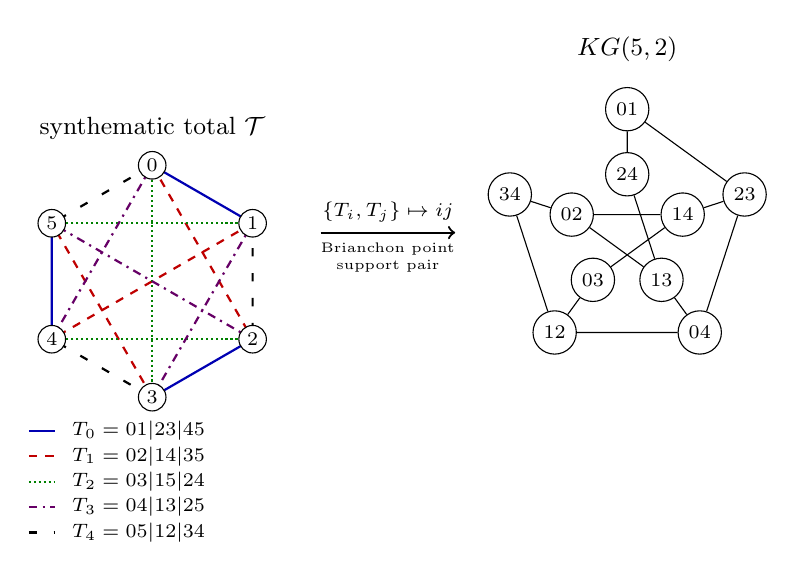
\begin{tikzpicture}[scale=0.95,
  vertex/.style={circle,draw,fill=white,inner sep=1.4pt,font=\scriptsize},
  pvertex/.style={circle,draw,fill=white,minimum size=5.5mm,inner sep=0pt,
                  font=\scriptsize}]
  % The invariant one-factorization on the six coordinate positions.
  \foreach \i/\a in {0/90,1/30,2/-30,3/-90,4/-150,5/150}
    \coordinate (v\i) at (\a:1.55);
  \draw[blue!70!black,thick] (v0)--(v1) (v2)--(v3) (v4)--(v5);
  \draw[red!75!black,thick,dashed] (v0)--(v2) (v1)--(v4) (v3)--(v5);
  \draw[green!50!black,thick,densely dotted] (v0)--(v3) (v1)--(v5) (v2)--(v4);
  \draw[violet!80!black,thick,dash dot] (v0)--(v4) (v1)--(v3) (v2)--(v5);
  \draw[black,thick,loosely dashed] (v0)--(v5) (v1)--(v2) (v3)--(v4);
  \foreach \i in {0,...,5} \node[vertex] at (v\i) {\i};
  \node[font=\small] at (0,2.05) {synthematic total $\mathcal T$};
  \begin{scope}[yshift=-2.0cm,font=\scriptsize]
    \draw[blue!70!black,thick] (-1.65,0)--(-1.3,0);
    \node[anchor=west] at (-1.2,0) {$T_0=01|23|45$};
    \draw[red!75!black,thick,dashed] (-1.65,-.34)--(-1.3,-.34);
    \node[anchor=west] at (-1.2,-.34) {$T_1=02|14|35$};
    \draw[green!50!black,thick,densely dotted] (-1.65,-.68)--(-1.3,-.68);
    \node[anchor=west] at (-1.2,-.68) {$T_2=03|15|24$};
    \draw[violet!80!black,thick,dash dot] (-1.65,-1.02)--(-1.3,-1.02);
    \node[anchor=west] at (-1.2,-1.02) {$T_3=04|13|25$};
    \draw[black,thick,loosely dashed] (-1.65,-1.36)--(-1.3,-1.36);
    \node[anchor=west] at (-1.2,-1.36) {$T_4=05|12|34$};
  \end{scope}

  \draw[->,thick] (2.25,.65)--(4.05,.65)
    node[midway,above,font=\scriptsize] {$\{T_i,T_j\}\mapsto ij$}
    node[midway,below,align=center,font=\tiny] {Brianchon point\\support pair};

  % Petersen graph on the two-subsets of {0,1,2,3,4}; adjacency is disjointness.
  \begin{scope}[xshift=6.35cm,yshift=.65cm]
    \node[pvertex] (p01) at (90:1.65) {01};
    \node[pvertex] (p23) at (18:1.65) {23};
    \node[pvertex] (p04) at (-54:1.65) {04};
    \node[pvertex] (p12) at (-126:1.65) {12};
    \node[pvertex] (p34) at (162:1.65) {34};
    \node[pvertex] (p24) at (90:.78) {24};
    \node[pvertex] (p14) at (18:.78) {14};
    \node[pvertex] (p13) at (-54:.78) {13};
    \node[pvertex] (p03) at (-126:.78) {03};
    \node[pvertex] (p02) at (162:.78) {02};
    \draw (p01)--(p23)--(p04)--(p12)--(p34)--cycle;
    \draw (p01)--(p24) (p23)--(p14) (p04)--(p13)
          (p12)--(p03) (p34)--(p02);
    \draw (p24)--(p13)--(p02)--(p14)--(p03)--cycle;
    \node[font=\small] at (0,2.45) {$KG(5,2)$};
  \end{scope}
\end{tikzpicture}
\caption{The synthematic--Petersen dictionary. The five line styles encode
the five self-polar triangles as perfect matchings of the six coordinates.
For each pair $\{T_i,T_j\}$, their union is an alternating six-cycle: its
opposite-edge matching gives a Brianchon point, and its alternating vertex
classes give a complementary support pair. Both are represented by the
Petersen vertex $ij$; adjacency means that the index pairs are disjoint.}
\label{fig:synthematic-petersen}
\end{figure}

\begin{proposition}[Brianchon--support dictionary]
\label{prop:brianchon-support}
Let $\mathcal T$ be the five self-polar triangles of Edge and
Dye~\cite{Edge1956,Dye1991}, regarded as the five perfect matchings in
their synthematic total, and let $\mathcal B(A)$ be the set of ten
Brianchon points of the Clebsch hexagon. For distinct $T,T'\in\mathcal T$,
the union $T\cup T'$ is an alternating six-cycle. Let $M(T,T')$ be the
perfect matching joining opposite vertices of this cycle. Let
$\beta(T,T')=\{S,S^{\mathsf c}\}$ be the unordered pair of alternating
vertex classes of the cycle.
For example, $T_0\cup T_1$ is the cycle
$0,1,4,5,3,2$, so $M(T_0,T_1)=05|13|24$ and
$\beta(T_0,T_1)=\{\{0,3,4\},\{1,2,5\}\}$.

The three chords indexed by $M(T,T')$ concur at a point $b(T,T')\in
\mathcal B(A)$. The maps
\[
 \binom{\mathcal T}{2}\longrightarrow\mathcal B(A),
 \qquad \{T,T'\}\longmapsto b(T,T'),
\]
and
\[
 \binom{\mathcal T}{2}\longrightarrow
 \bigl\{\{S,S^{\mathsf c}\}:|S|=3\bigr\},
 \qquad \{T,T'\}\longmapsto\beta(T,T'),
\]
are $A_5$-equivariant bijections. They identify the ten Brianchon points
with the ten complementary support pairs. Under this identification,
Petersen adjacency is disjointness of the corresponding two-element
subsets of $\mathcal T$.
\end{proposition}

\begin{proof}
The opposite-vertex matching is disjoint from $T$ and $T'$ and contains
one edge from each of the other three members of the synthematic total.
Hence $\{T,T'\}$ is recovered as the two members of $\mathcal T$ disjoint
from $M(T,T')$, so the ten triangle pairs give exactly the ten perfect
matchings outside the total. Applying the alternating-class rule to the
five displayed matchings gives ten distinct complementary support pairs,
hence all ten such pairs. Edge's Clebsch construction says that the
three chords of each such matching concur, at the ten distinct Brianchon
points~\cite[\S\S19--20,30]{Edge1956}. The bipartition bijection and
Petersen assertion are the alternating-cycle construction above.

The ten outside matchings give the ten triple concurrences. The remaining
fifteen intersections of disjoint chords have multiplicity one. Since every
step uses only the invariant total and incidence, both bijections and their
compatibility with the support map are $A_5$-equivariant.
\end{proof}

\begin{corollary}[The decoder reconstructs the Brianchon configuration]
\label{cor:decoder-brianchon}
The ten projective directions having three nearest weight-two errors are
exactly the ten Brianchon points.  At each such direction the three error
supports are pairwise disjoint and hence form a perfect matching of the six
coordinates.  The ten matchings thereby recovered are precisely the ten
perfect matchings outside the five-matching synthematic total.
\end{corollary}

\begin{proof}
The three weight-two representations of a secant-index-three direction use
the three chords through it.  Proposition~\ref{prop:brianchon-support}
identifies the ten triple concurrences with the ten Brianchon points and
their chords with exactly the ten matchings complementary to the total.
\end{proof}

\begin{proposition}[Invariant support bipartition]
\label{prop:chirality}
Only the bipartition is intrinsic: neither part has a canonical sign. The
twenty three-element coordinate supports split into two complementary
$A_5$-orbits $\mathcal O_+$ and $\mathcal O_-$ of size ten. For every
maximum-distance syndrome $s$, each support determines exactly one
weight-three leader of the coset $H^{-1}(s)$; hence that coset has ten
leaders supported in each class. Globally, the $2400$ minimum-weight
leaders split as $1200+1200$.

Every monomial automorphism of $C$ preserves this unordered bipartition.
The other coset in the exotic normalizer $N_{S_6}(A_5)\cong S_5$ exchanges
the two support classes, but its sixty elements are not automorphisms of the
displayed code. By
Proposition~\ref{prop:brianchon-support}, the ten complementary support
pairs are canonically both the two-subsets of the five self-polar triangles
and the ten Brianchon points.
\end{proposition}

\begin{proof}
The degree-six action of $A_5$ on the twenty three-subsets has two
ten-element orbits, exchanged by complementation. It preserves a unique
synthematic total, also preserved by
its full $S_5$ normalizer. The alternating-cycle construction of
Figure~\ref{fig:synthematic-petersen} is therefore equivariant, and the
outside normalizer coset exchanges the two support orbits. Fix a
maximum-distance syndrome $s$ and a three-support $S$. The three columns
indexed by $S$ are independent because $A$ is an arc, so they give a unique
coefficient vector representing $s$. None of its three coefficients can
vanish: otherwise $[s]$ would lie on a secant of $A$, contrary to maximum
distance. The resulting error vector therefore has weight three and is the
unique leader with support $S$. Finally, every monomial automorphism induces
a support permutation in $A_5$, by the exact sequence in
Section~\ref{sec:automorphisms}, and so preserves each support orbit. The
outside normalizer coset swaps the two orbits but cannot preserve $C$, even
after coordinate rescaling, because its support permutations lie outside
that quotient $A_5$.
\end{proof}

\section{Why \texorpdfstring{$q=11$}{q=11}}
\label{sec:why11}

Call an arc $A$ \emph{conic-filling} if $\cU(A)=\mathcal Q(\F_q)$ for some
nonsingular conic $\mathcal Q$. The conic-filling syndrome phenomenon of
Sections~\ref{sec:code}--\ref{sec:rigidity} is specific to $q=11$, even
without a symmetry hypothesis on the arc. A universal chord-multiplicity
identity makes this a four-field question, and the only nontrivial residue
is a classical exact-distance problem in the Sylvester graph.

\begin{lemma}[Chord-defect identity]
\label{lem:chord-defect}
Let $A$ be a six-arc in $\PG(2,q)$, and let $c(A)$ be the number of points
off $A$ incident with three of its fifteen chords. Then
\[
 |\cU(A)|=q^2-14q+55-c(A),\qquad 0\le c(A)\le15.
\]
Consequently, if $|\cU(A)|=q+1$, then
\[
 c(A)=(q-6)(q-9).
\]
\end{lemma}

\begin{proof}
At a point off $A$, concurrent chords have pairwise disjoint endpoint
pairs, so at most three chords occur. Let $n_i$ count the off-arc points on
exactly $i$ chords. Counting chord--point incidences and pairs of chords
with disjoint endpoints gives
\[
 n_1+2n_2+3n_3=15(q-1),\qquad
 n_2+3n_3=\binom{15}{2}-6\binom{5}{2}=45.
\]
Writing $c(A)=n_3$, the number of covered points off $A$ is
$n_1+n_2+n_3=15q-60+c(A)$. Subtracting this from the
$q^2+q-5$ points off $A$ proves the identity. Each triple concurrence
uses one of the fifteen perfect matchings of the six endpoints, and a fixed
matching can be concurrent at only one point; hence $c(A)\le15$. The last
display follows on setting $|\cU(A)|=q+1$.
\end{proof}

\begin{theorem}[Uniqueness of $q=11$]
\label{thm:why11}
Let $q$ be a prime power. If a six-arc $A\subset\PG(2,q)$ satisfies
$\cU(A)=\cC(\F_q)$ for some nonsingular conic $\cC$, then $q=11$.
At $q=11$ every such $A$ is projectively equivalent to the
Clebsch hexagon.
\end{theorem}

\begin{proof}
Lemma~\ref{lem:chord-defect} gives
$c(A)=(q-6)(q-9)$ with $0\le c(A)\le15$. The prime-power condition therefore
leaves only $q\in\{4,5,9,11\}$: the values at $7$ and $8$ are negative,
while every integer $q\ge12$ gives $c(A)\ge18$.

At $q=4$, every six-arc is a hyperoval. Each point off it lies on three
secants (count the six hyperoval points on the five lines through the
point), so $\cU(A)$ is empty. At $q=5$, every six-arc is an oval and hence a
nonsingular conic; the standard internal/external point counts show that
every off-conic point lies on a secant, so again $\cU(A)$ is empty.

It remains to exclude $q=9$. The argument has three steps: the six arc
points must be internal to $\cC$; passant joins of internal points become
distance-two pairs in the Sylvester graph; and that distance graph has
clique number five. Since every point of $\cC$ is uncovered, no chord of
$A$ meets $\cC$; every chord is therefore passant. A point off $\cC$ lies on five passants if it
is internal and four if it is external; hence the five chords through each
vertex force all six vertices of $A$ to be internal. Let $\Sigma$ be the graph
on the $36$ internal points, with $P\sim Q$ when $Q\in P^\perp$ under the
conic polarity. Standard conic counts give the intersection array
\[
 \{5,4,2;1,1,4\},
\]
so $\Sigma$ is the Sylvester graph
\cite[\S13.1.2]{BrouwerCohenNeumaier1989}; see also the combinatorial
uniqueness proof in~\cite[Thm.~6]{JurisicVidali2019}. For distinct internal
points, the unique possible common neighbor is
$P^\perp\cap Q^\perp=(PQ)^\perp$; consequently $PQ$ is passant exactly when
$P,Q$ are at distance two in $\Sigma$. Thus $A$ would be a six-clique in the
graph joining pairs at distance exactly two in $\Sigma$. But its clique number, denoted
$\operatorname{eq}_2(\Sigma)$ in
\cite[Table~1]{AbiadJabalAmeliReijnders2025}, is five, a contradiction.

Therefore $q=11$. The final assertion follows from
Theorem~\ref{thm:rigidity}, which puts every matching $q=11$ representative
in the single Clebsch orbit.
\end{proof}

\begin{proposition}[The Clebsch-family uncovered formula]
\label{prop:clebsch-family-uncovered}
Let $K$ be a Clebsch hexagon over $\F_q$. Then
\[
 |\cU(K)|=q^2-14q+45.
\]
If $q\equiv3\pmod4$ and $\cC$ is Dye's associated conic, then
$\cC(\F_q)\subseteq\cU(K)$ and
\[
 |\cU(K)\setminus\cC(\F_q)|=(q-4)(q-11).
\]
In particular, among Clebsch hexagons in this congruence class, the
associated conic is the complete projective deep-hole syndrome locus if and
only if $q=11$.
\end{proposition}

\begin{proof}
Dye defines a Clebsch hexagon by the occurrence of exactly ten Brianchon
points, and his Theorem~1 classifies their existence and projective orbit
\cite[p.~271; Theorem~1, pp.~275--276]{Dye1991}. These points are precisely the off-vertex
triple-chord concurrences counted by $c(K)$. Thus $c(K)=10$, and
Lemma~\ref{lem:chord-defect} gives
\[
 |\cU(K)|=q^2-14q+55-10=q^2-14q+45.
\]
Dye also shows that the edges of $K$ are non-secants of the associated conic
when $q\equiv3\pmod4$~\cite[discussion preceding Theorem~6,
pp.~281--282]{Dye1991}. Hence every rational point of $\cC$ is uncovered.
Subtracting $|\cC(\F_q)|=q+1$ from the first formula gives
\[
 q^2-15q+44=(q-4)(q-11).
\]
The factor vanishes only at $q=4$ and $q=11$, and the stated congruence
leaves only $q=11$. Conversely, Clebsch hexagons exist over $\F_{11}$ by
Dye's Theorem~1, and the inclusion above is then an equality because both
sets have twelve points.
\end{proof}

\begin{remark}[The next admissible field]
At $q=19$, the same icosahedral construction still produces a Clebsch
six-arc disjoint from its associated conic, but the covering fails. The
twenty conic points remain uncovered~\cite[p.~281]{Dye1991}, while
Proposition~\ref{prop:clebsch-family-uncovered} gives
\[
 |\cU(A)|=140=20+120.
\]
Thus $120=(19-4)(19-11)$ additional points escape all fifteen secants, and
$\cU(A)$ lies on no conic. The configuration persists; exact conic filling
is what the factorization isolates at $q=11$.
\end{remark}

\subsection{The two reflection-arrangement exceptions}
\label{sec:reflection-exceptions}

The chord moments below classify the neighboring arc sizes. The two
survivors have a common arrangement-theoretic organization, although the
arrangement calculation alone gives complement sizes, not conic equations.

Let $F$ be a field of characteristic different from two containing
$\tau$ with $\tau^2=\tau+1$. In dual coordinates, take the fifteen line
normals
\[
 (1,0,0),(0,1,0),(0,0,1),\qquad
 \operatorname{cyc}(1,\epsilon\tau,\delta(\tau-1))
 \quad(\epsilon,\delta\in\{\pm1\}).
\]
Over the real embedding with $\tau=(1+\sqrt5)/2$, their signed versions
are the roots of type $H_3$; over other fields this denotes the displayed
finite reduction of the icosahedral mirror arrangement.

\begin{proposition}[The Clebsch secants as reduced $H_3$ mirrors]
\label{prop:h3-arrangement}
The six fivefold points are
\[
 (0,1,1-\tau),(0,1,\tau-1),(1,1-\tau,0),(1,\tau-1,0),
 (1,0,-\tau),(1,0,\tau).
\]
They form an arc, their fifteen joins are the mirrors, and the other
singularities are ten triple and fifteen double points. Over $\F_{11}$,
take $\tau=8$. The matrix
\[
 T=\begin{pmatrix}2&3&8\\10&6&9\\2&2&5\end{pmatrix}
\]
maps these six column vectors onto the displayed Clebsch hexagon $A$.
Writing line coefficients as rows, the induced map
$\ell\mapsto\ell T^{-1}$ carries the mirrors onto the secants of $A$.
\end{proposition}

\begin{proof}
Pairwise cross-products of the normals give the stated
$6_5,10_3,15_2$ ledger, and joining the six fivefold points recovers all
fifteen normals. These are symbolic identities in
$R=\mathbb Z[\tau]/(\tau^2-\tau-1)$, obtained by reducing each coordinate
to $a+b\tau$. In the same ring, every three-by-three determinant on the six
points is $2u$ for some $u\in R^\times$. Under any specialization
$R\to F$, the image of $u$ remains a unit and the image of $2$ is nonzero
when $\operatorname{char}F\ne2$; hence the six points remain an arc.
Finally, $\det T=3$ in $\F_{11}$ and direct multiplication gives the two
asserted set equalities.
\end{proof}

Characteristic two is bad because the signs coalesce. In every other
characteristic containing $\tau$, the displayed mirror-intersection
lattice survives.  The stronger ``lattice-good'' condition used in
Theorem~\ref{thm:headline-rigidity-phase}(A2) also prevents new
collinearities among its singular points and is defined in
Proposition~\ref{prop:lattice-good}. In
characteristic five, the reflection group $W(H_3)$ has order $120$, which
is divisible by the characteristic, so the modular group algebra is not
semisimple. This does not collapse the coordinate arrangement:
at $\tau=3\in\F_5$, the fifteen distinct mirrors and the full
$6_5,10_3,15_2$ ledger remain. The finite checks for this statement and the
$\F_{11}$ projectivity are recorded in
Section~\ref{sec:verification}. For the central rank-three hyperplane
arrangement, a point where $m$ projective mirrors meet has M\"obius value
$m-1$. Thus
\[
 \chi_{H_3}(t)=t^3-15t^2+59t-45=(t-1)(t-5)(t-9).
\]
Dividing the affine complement count by $q-1$ gives $(q-5)(q-9)$
projective points. At $q=11$, the points lying on respectively zero, one,
two, and three mirrors number $12,90,15,10$; here ``one'' means an
ordinary mirror point. With the six fivefold points marked as columns,
these are exactly the projective strata behind
Proposition~\ref{prop:decoding-oracle}; the general passage to
coset-leader multiplicities is due to Jurrius and
Pellikaan~\cite{JurriusPellikaan2015}.

For the standard four-frame $E=\{e_1,e_2,e_3,(1,1,1)\}$, the six joins
have equations
\[
 X,Y,Z,X-Y,X-Z,Y-Z=0.
\]
These are the essentialized braid mirrors $x_i=x_j$ of type $A_3$, after
setting $x_4=0$. Their four triple and three double points give
\[
 \chi_{A_3}(t)=(t-1)(t-2)(t-3),\qquad
 |\PG(2,q)\setminus\textstyle\bigcup A_3|=(q-2)(q-3).
\]
In the faithful-reduction range just stated for the explicit $H_3$ model,
the two size equations are therefore
\[
\begin{array}{c@{\quad}c@{\quad}c}
\text{arc}&\text{secant arrangement}&|\cU|=q+1\\ \hline
\text{four-frame}&A_3&(q-1)(q-5)=0\\
\text{Clebsch hexagon}&H_3&(q-4)(q-11)=0.
\end{array}
\]
The extraneous root $q=4$ lies precisely in the bad characteristic-two
regime, where the displayed $H_3$ reduction degenerates. Thus, in the
faithful-reduction range, the arrangement factorizations leave precisely
$q=5$ and $q=11$.

\subsection{The common Coxeter-number calculation}
\label{sec:coxeter-number-phase}

The preceding $A_3$ and $H_3$ calculations are the end members of one
rank-three argument.  For $B_3$ use the nine normals
\[
 X,Y,Z,\quad X\mathbin{\pm}Y,\quad X\mathbin{\pm}Z,\quad
 Y\mathbin{\pm}Z .
\]
We first make the reduction hypothesis precise.  For $A_3$ and $B_3$ let
$R_T=\mathbb Z[1/2]$; for $H_3$ let
\[
 R_{H_3}=\mathbb Z[\tau,1/2]/(\tau^2-\tau-1)
\]
and use the fifteen displayed normals of
Proposition~\ref{prop:h3-arrangement}.  Write $\mathcal A_T$ for the
arrangement over the fraction field of $R_T$, and $\mathcal S_T$ for its
rank-two flats, represented by primitive vectors $x_P\in R_T^3$.
Form the following finite list, omitting a determinant exactly when it is
zero over the fraction field:
\[
\begin{split}
 &n_i,\quad n_i\wedge n_j,\quad
   \det(n_i,n_j,n_k)\ \text{when this determinant is nonzero},\\
 &x_P,\quad x_P\wedge x_{P'},\quad
   \det(x_P,x_{P'},x_{P''})\
   \text{when this determinant is nonzero}.
\end{split}                                                   \tag{7.1}
\]

\begin{proposition}[Lattice-good reduction]
\label{prop:lattice-good}
A specialization $\varphi:R_T\to\F_q$ is \emph{lattice-good} if
$\varphi$ sends every vector in (7.1) to a nonzero vector and every listed
determinant to a nonzero scalar.  These are finitely many explicit
polynomial nonvanishing conditions.  Characteristic two is excluded, and an
$H_3$ specialization includes a chosen
$\varphi(\tau)\in\F_q$ satisfying $\varphi(\tau)^2-\varphi(\tau)-1=0$.
Under this condition:
\begin{enumerate}[label=\textup{(\roman*)},leftmargin=*]
\item the reduced normals define the same number of distinct mirrors, the
same rank-three intersection lattice, and the same singular
multiplicities as $\mathcal A_T$;
\item the weighted collinearity matroid of the singular points is
unchanged.  In particular, for nonmirror lines
\[
 \max_L\sum_{P\in L\cap\mathcal S_T}(m(P)-1)=h/2;
\]
\item if the complement is nonempty, it spans $\PG(2,q)$.
\end{enumerate}
\end{proposition}

\begin{proof}
The first line of (7.1) preserves nonzero normals, distinct mirror
directions, and the zero pattern of every three-normal determinant.
Hence it preserves rank and the complete intersection lattice.  The
second line preserves distinct singular points and the zero pattern of
every determinant of three such points.  It therefore preserves every
line containing at least two singular points, together with the
multiplicities used in its weight.  A line containing at most one
singular point has weight at most the largest single value $m(P)-1$.
The characteristic-zero ledgers below have maxima $2,3,5=h/2$; these
maxima and the lines attaining them consequently survive unchanged.

The complement count proved below is
$(q-h/2)(q-h+1)$.  In a lattice-good specialization, nonemptiness forces
$q>h-1$ in the three displayed types (the smaller $H_3$ fields admitting
$\tau$ are $\F_5$ and $\F_9$, where the count is zero).  Its size is
therefore strictly greater than the maximum $q-h+1$ on one line.  The
complement is not collinear and its evaluation code has dimension three.
\end{proof}

Put $e=h/2$ and $N=3h/2$.  The relevant intersection data are
\[
\begin{array}{c|c|c|c}
T&(1,e,h-1)&N&\text{projective singular flats}\\ \hline
A_3&(1,2,3)&6&3\text{ double},\ 4\text{ triple}\\
B_3&(1,3,5)&9&6\text{ double},\ 4\text{ triple},\ 3\text{ fourfold}\\
H_3&(1,5,9)&15&15\text{ double},\ 10\text{ triple},\ 6\text{ fivefold}.
\end{array}                                                    \tag{7.2}
\]
Thus the finite-field method, equivalently inclusion along the flats in
(7.2), gives
\[
 |B_T(q)|=(q-e)(q-h+1).                              \tag{7.3}
\]

Here is the common distance mechanism.  If $L$ is not a mirror, define
\[
 \delta(L)=\sum_{\substack{P\in L\\P\text{ singular}}}(m(P)-1),
\]
where $m(P)$ is the number of mirrors through $P$.  The $N$ mirror
intersections on $L$ are distinct except for precisely these collisions,
so
\[
 |L\cap B_T(q)|=q+1-N+\delta(L).                     \tag{7.4}
\]
Proposition~\ref{prop:lattice-good} transports the exact singular-line
ledgers and gives
\[
 \max_{L\ {\rm nonmirror}}\delta(L)=e
\]
in all three types: the maxima are respectively $2,3,5$.  Consequently
(7.4) has maximum $q-h+1$.  A nonzero coefficient vector of the
dimension-three projective evaluation code vanishes exactly on the
intersection with its projective line.  Proposition~\ref{prop:lattice-good}
supplies dimension three.  Subtracting this maximum from (7.3) proves
\[
 D_T(q)=
 \bigl[(q-e)(q-h+1),\,3,\,(q-e-1)(q-h+1)\bigr]_q
                                                               \tag{7.5}
\]
whenever the complement is nonempty.  This proves
Theorem~\ref{thm:headline-rigidity-phase}(A2).

At $q=h+1$, the invariant form
\[
 Q=X^2+Y^2+Z^2
\]
is nonsingular.  For a mirror with pole $r$, externality to $Q$ is the
condition that $-Q(r)$ be a nonsquare.  The root-norm classes are
\[
\begin{array}{c|c|c}
T&q&Q(r)\text{ classes};\ -Q(r)\text{ classes}\\ \hline
A_3&5&\{2\};\ \{3\}\\
B_3&7&\{1,2\};\ \{6,5\}\\
H_3&11&\{1,4\};\ \{10,7\},
\end{array}
\]
and every class in the last column is nonsquare.  Hence every rational
point of $Q$ avoids every mirror.  Formula (7.3) gives
$|B_T(h+1)|=h+2=q+1$, so this containment is equality.  Evaluation on a
full nonsingular conic is the projective/extended GRS code
$[q+1,3,q-1]_q$, proving (A3).

Finally, in the same displayed coordinates the Coxeter transformations
have two rational eigenlines on the conic.  On the remaining affine
coordinate their squares act by generators of the square subgroup
$\F_q^{\times2}$, of order $(q-1)/2=h/2$.  They therefore generate the
split maximal torus of $\mathrm{PSL}_2(q)$ and partition the moving points
into the square and nonsquare, or Legendre, cosets.  The exact
characteristic polynomials and orders for $q=5,7,11$ are among the finite
checks in Section~\ref{sec:verification}; the identification of this
literal subgroup with the classical split torus uses the standard
subgroup classification~\cite{Giudici2007}.  This proves (A4).

\begin{theorem}[Conic-filling loci for $4\le k\le7$]
\label{thm:small-k-conic-filling}
Let $A$ be a $k$-arc in $\PG(2,q)$, where $q$ is a prime power and
$4\le k\le7$. If $\cU(A)$ is the full set of $\F_q$-rational points of a
nonsingular conic, then
\[
 (k,q)=(4,5)\qquad\text{or}\qquad(k,q)=(6,11).
\]
In the first case $A$ is a projective four-frame; in the second it is a
Clebsch hexagon. Conversely, both cases occur.
\end{theorem}

\begin{proof}[Proof with exhaustive finite verification]
Let $n_i$ count off-arc points incident with exactly $i$ chords. For
$k\le7$, at most three pairwise disjoint chords concur. Counting
chord--point incidences and pairs of disjoint chords gives the two universal
moments
\[
 \sum_i i n_i=\binom{k}{2}(q-1),\qquad
 \sum_i\binom{i}{2}n_i=3\binom{k}{4}.
\]
For $k=4$, every arc is a projective frame, so the $A_3$ calculation above
gives $|\cU(A)|=(q-2)(q-3)$. Equating this with $q+1$ gives $q=5$; for the
standard frame a direct substitution further gives
\[
 \cU(A)=V(X^2+Y^2+Z^2+XY+XZ+YZ),
\]
where $V(f)$ denotes the projective zero set of $f$; this is a nonsingular
six-point conic. For $k=5$, the same moments force
$n_2=15$ and $|\cU(A)|=q^2-9q+21$; equality with $q+1$ would require
$q^2-10q+20=0$, which has no integral root. The case $k=6$ is
Theorem~\ref{thm:why11} together with Theorem~\ref{thm:rigidity}.

For $k=7$, the moments give
\[
 |\cU(A)|=q^2-20q+120-n_3.
\]
If this equals $q+1$, then
\[
 n_3=q^2-21q+119,\quad
 n_2=105-3n_3,\quad
 n_1=3(q^2-14q+42).
\]
The standard arc-size bound gives $q\ge7$.  The condition $n_2\ge0$ gives
$q\le15$, so the prime-power candidates are
$q\in\{7,8,9,11,13\}$; then $n_1\ge0$ eliminates $7,8,9$.
Thus only $q=11$ and $q=13$ remain, with forced spectra
$(n_1,n_2,n_3)=(27,78,9)$ and $(87,60,15)$ respectively. An exhaustive
four-frame-normalized enumeration now supplies the finite exclusion. It
finds $10232$ distinct normalized seven-arcs at $q=11$, of which $140$ have
$|\cU(A)|=q+1$, and $53960$ at $q=13$, of which $1680$ have that size.
Every seven-arc is reached because it contains a four-frame; extending each
normalized six-arc by its uncovered points produces every resulting
seven-arc exactly three times, according to which non-frame point is
deleted. For all $1820$ candidates of the required size, the quadratic
evaluation matrix has full rank six, so none lies on a conic.
\end{proof}

For $k\ge8$ the second moment leaves additional concurrency parameters, so
the analogous classification remains open.

\section{Factorization memory in the conic ideal}
\label{sec:factorization}

Write the standard conic as $Q=XZ-Y^2$ and parametrize it by
$\nu(s:t)=(s^2:st:t^2)$.  For $a=(a_0:a_1)$ and $b=(b_0:b_1)$ on
$\PG(1,q)$, let $L_{ab}$ denote the secant through $\nu(a),\nu(b)$, scaled
so that
\[
 L_{ab}(\nu(s:t))=[a,(s:t)]\,[b,(s:t)],
 \qquad
 [a,b]=a_0b_1-a_1b_0.
\]
Let $\Omega$ be any set of $2m$ distinct conic points, with fixed vector
representatives, and for a perfect matching $M$ of $\Omega$ put
$P_M=\prod_{\{a,b\}\in M}L_{ab}$.

\begin{proposition}[The matching-secant quotient]
\label{prop:general-matching-quotient}
For every $m\ge2$ and every pair of perfect matchings $M,N$ of $\Omega$,
\[
 P_M|_Q=P_N|_Q,\qquad P_M-P_N\in(Q).
\]
Consequently, after choosing a reference matching $M_0$,
\[
 \Phi_{M_0}(M)=\frac{P_M-P_{M_0}}{Q}
       \in H^0(\mathbb P^2,\mathcal O(m-2))                 \tag{8.1}
\]
is an affine configuration.  Replacing $M_0$ by $M_1$ translates it by
$-\Phi_{M_0}(M_1)$.  If $g\in\mathrm{GL}_2$ preserves $\Omega$,
$\rho(g)$ is its action on binary quadratics, and representatives are
transported by $g$, then
\[
 \Phi_{gM_0}(gM)\circ\rho(g)
   =\det(g)^{\,2m-2}\Phi_{M_0}(M).                          \tag{8.2}
\]
Thus the difference space, its rank, and its affine moment conditions are
independent of $M_0$ and equivariant under the endpoint stabilizer.
\end{proposition}

\begin{proof}
For $x\in\mathbb P^1$,
\[
 P_M(\nu(x))=\prod_{a\in\Omega}[a,x],
\]
which is independent of the pairing.  The kernel of the Veronese pullback
$k[X,Y,Z]\to k[s,t]$, $(X,Y,Z)\mapsto(s^2,st,t^2)$, is the principal
ideal $(Q)$; hence every difference is divisible by $Q$.  The change of
reference follows by subtraction.  Finally,
$L_{ga,gb}\circ\rho(g)=\det(g)^2L_{ab}$ and
$Q\circ\rho(g)=\det(g)^2Q$, which gives (8.2).
\end{proof}

For four endpoints, the Pl\"ucker relation makes the divisibility
especially concrete:
\[
 L_{ab}L_{cd}-L_{ac}L_{bd}
   =[a,d][b,c]\,Q.                                      \tag{8.3}
\]
The formal development checks this four-endpoint identity and
arbitrary-size switch reversibility.  Proposition
\ref{prop:general-matching-quotient} is the general human proof; it does
not assert that a selected finite Coxeter orbit contains every perfect
matching.

For the Coxeter applications, fix a reference matching $M_0$ and write
\[
 \Phi(M)=\frac{P_M-P_{M_0}}{Q}.
\]
Changing $M_0$ translates every point by the same vector, so affine moment
statements and difference ranks are independent of that choice.  Kernel
reduction of the three displayed Coxeter matching orbits gives
\[
\begin{array}{c|ccc}
 &A_3&B_3&H_3\\ \hline
\text{matching-orbit size}&5&14&22\\
\operatorname{rank}\langle\Phi(M)-\Phi(N)\rangle&3&6&10.
\end{array}                                             \tag{8.4}
\]
The symbolic conic Laplacian decomposes the degree-$1,2,4$ homogeneous
pieces into harmonic and radial parts at the stated characteristics; (8.3)
is the bridge placing switch differences in the radial summand.  The
symbolic dimension formulas do not imply the finite factorization-image
ranks in (8.4); those ranks require the displayed coordinate calculation.

\paragraph{Proof of Theorem \ref{thm:headline-factorization}(F1).}
The pullback formula and Pl\"ucker identity prove the divisibility statement.  The generic
augmentation-kernel calculation controls the one-dimensional translation
lost by choosing $M_0$.  Exact row reduction of the three coordinate
configurations gives (8.4), proving the rank statement.  The trust table in
Section~\ref{sec:verification} separates the symbolic identity, the
kernel-checked finite ranks, and the classical identification of the
coordinate orbits with the named Coxeter matchings.

\section{Balanced sheets and cubic-first orientation}
\label{sec:balanced}

Let $\Omega=\Omega_+\sqcup\Omega_-$ be the $B_3$ or $H_3$
factorization orbit, with $|\Omega_+|=|\Omega_-|=q$, and let
$x_\omega=\Phi(\omega)$.  For a signed weight
$\epsilon=+1$ on $\Omega_+$ and $-1$ on $\Omega_-$, define a scalar shadow
of the $j$th signed tensor moment by
\[
 M_j(\ell)=\sum_{\omega\in\Omega}
   \epsilon(\omega)\,\ell(x_\omega)^j .
\]
For $j\le3$ over the working fields $\F_7$ and $\F_{11}$, polarization is
valid because $j!$ is invertible.  Thus the symmetric tensor moment is
zero exactly when all its scalar pure-power shadows $M_j(\ell)$ vanish.
An affine change $x\mapsto Ax+c$ changes the first surviving degree-$j$
moment by $A^{\otimes j}$; lower vanishing removes the translation.

The degree-two recovery is most transparent in the function space on the
two sheets.  Let $L$ be the affine-evaluation subspace and $L^{\circ2}$ the
span of coordinatewise products of pairs of functions in $L$.  The finite
decoders on each sheet prove
\[
 L^{\circ2}=
 \left\{(u,v):\sum_{\Omega_+}u=\sum_{\Omega_-}v\right\}. \tag{9.1}
\]
The target is a codimension-one subspace of the $2q$-dimensional function
space, hence has dimension $13$ for $B_3$ and $21$ for $H_3$.  For the
forward inclusion, equality of the two sheet sums is checked on every
product of affine evaluations and hence on their span.  Conversely, the
finite decoders show that $L$ restricts surjectively onto the zero-sum
hyperplane on each sheet (dimensions $6$ and $10$), contains both sheet
indicators, and contains a product with nonzero common sheet sum.  These
three facts generate the two zero-sum summands and one remaining common-sum
direction, proving the reverse inclusion in (9.1).
The annihilator of the hyperplane on the right is the line spanned by the
sheet-sign vector.  Therefore a pointwise $\{\pm1\}$ weight annihilates all
quadratic products precisely when it is the sheet sign or its negative.
This proves that the two displayed sheets are the unique balanced
complementary halves, up to interchange.

An involution exchanges $\Omega_+$ and $\Omega_-$ and negates the six
compressed profile vectors.  Consequently every even signed profile
moment vanishes.  On the positive profiles the primitive relation is
\[
 v_1+4v_4+6v_6=0,                                      \tag{9.2}
\]
which kills the signed barycentre.  A displayed cubic coordinate is
nonzero in both the $B_3$ and $H_3$ configurations.  Hence degrees one and
two vanish while degree three survives.  This is the exact meaning of
``cubic-first'': it concerns signed tensor moments and their linear
functionals, not all conceivable invariants.

The signed cubic is fixed by the subgroup preserving each sheet and
negated by the outer generator.  The finite affine-action checks, together
with nonvanishing, identify its stabilizer inside the displayed generated
action with the kernel of the sign character.  Identifying that generated
action with the classical $\mathrm{PSL}_2(q)$ subgroup of
$\mathrm{PGL}_2(q)$ is a named group-theoretic input.

\paragraph{Proof of Theorem \ref{thm:headline-factorization}(F2--F3).}
Equation (9.1) and its annihilator calculation prove balanced uniqueness.
The antipodal identity and (9.2) prove the even and linear cancellations.
For the displayed profile coordinate, the first possible odd survivor is
\[
  2\bigl((-6)^3+4(-3)^3+6(3)^3\bigr)=6\ne0\pmod {11},
\]
so degree three survives.  The relative-invariant lemma gives the kernel
stabilizer.  All statements remain valid after an affine change of the
quotient coordinates by the first-survival formula.

\section{Six depth profiles and matching-row reconstruction}
\label{sec:depth}

Put $G=\mathrm{PGL}_2(11)$, let $H=A_5$ stabilize one $H_3$ matching, and
let $K=A_4$ be the common subgroup selected by an edge decoration.  The
finite two-sided action has six $K$--$H$ relation cells.  Its $K$-orbits
on each $H$-sheet have sizes $1,4,6$.  One secant-incidence recount on a
representative of each cell gives the six distinct profiles
\[
 v_1,\ v_4,\ v_6,\ -v_1,\ -v_4,\ -v_6.                \tag{10.1}
\]
Their coordinates are
\[
\begin{aligned}
v_1&=(-6,0,12,-12),\\
v_4&=(-3,3,0,3),\\
v_6&=(3,-2,-2,0).
\end{aligned}
\]
The subscripts record the orbit sizes.  The four coordinates are signed
differences of zero counts on the oriented relation pairs
$(R_1,R_{10})$, $(R_3,R_{13})$, $(R_6,R_{14})$, and
$(R_9,R_{11})$.  For example, the positive singleton has zero-count row
\[
 (0,6;\ 0,0;\ 12,0;\ 0,12),
\]
whose four differences give $v_1$.  Reversing every oriented pair gives
the negative singleton and the profile $-v_1$.  The other two positive
orbits have sizes four and six and give $v_4$ and $v_6$; the opposite
sheet gives their negatives.

The positive three satisfy (9.2) and two plane equations.  The resulting
linear map from the six relation indicators has rank two and kernel
dimension four, but (10.1) shows that its restriction to the set of six
labels is injective.  Linear rank loss therefore does not imply loss of the
finite label.

The singleton cells supply the reconstruction.  The positive and negative
singletons identify the two $H_3$ matching rows, so without a choice the
profile data recover their unordered pair.  On the six displayed labels,
the recovery map is the inverse of (10.1):
\[
 v_1\longmapsto M_+,\qquad -v_1\longmapsto M_-,
\]
where $M_+$ and $M_-$ are the two singleton rows of the frozen matching
table.  Choosing
a sheet and its singleton therefore selects one decorated row.  The
kernel-checked terminal proves this finite table-row recovery; identifying
that row with a geometric Clebsch parent would require an additional
row-to-geometry bridge and is not claimed here.

The characteristic-eleven permutation module gives an intrinsic
explanation of the rank drop.  On one sheet the degree-eleven permutation
module is the projective cover $P(1)$ with Loewy dimensions $1\mid9\mid1$.
Its $A_4$-fixed space has orbit-sum basis of sizes $1,4,6$, and quotienting
by the all-ones socle gives precisely the depth plane.  The unique primitive
positive dependence of the three rays is $1:4:6$, so the rays themselves
recover both those orbit sizes and, by orbit--stabilizer, the orders
$12,3,2$.

\begin{proposition}[Modular depth quotient and source boundary]
\label{prop:modular-depth-plane}
Over $\F_{11}$ the depth plane is
\[
  P(1)^{A_4}/\operatorname{soc}P(1),\qquad
  \operatorname{Loewy}(P(1))=1\mid9\mid1.
\]
Separately, the three-dimensional relative-cubic invariant space $R$ and
its coinvariants $M_G$ have canonical maps
\[
 R\xrightarrow{\ \pi\ }M_G\xrightarrow{\ N\ }R
\]
of ranks two and one, with
$\operatorname{im}\pi=\ker N$ and
$\operatorname{im}N=\ker\pi=\langle[1:3:9]\rangle$.
Invariant-to-coinvariant projection and contraction by the unique
rank-one semi-invariant form therefore construct the same canonical Tate
two-plane.  This plane is not naturally identified with the depth plane:
the labelled cubic orbit classes have relation $[2,9,1]$, while the depth
profiles have relation $[2,8,1]$; divided transfer kills the former
balanced relations and fixes the latter socle.
\end{proposition}

\paragraph{Proof of Theorem \ref{thm:headline-factorization}(F4) and
Proposition~\ref{prop:modular-depth-plane}.}
The exact generator permutations partition all twenty-two matchings into
the six orbits of (10.1); the representative recounts are constant on
those orbits.  Row reduction gives the rank and kernel dimensions, and
direct comparison proves set-theoretic separation.  The two singleton
recovery maps give the unordered matching pair, after which the chosen
singleton returns its decorated row in the frozen table.  Projectivity,
the local two-dimensional commuting algebra, and exactness of
$A_4$-fixed points give the $1\mid9\mid1$ quotient: the $A_5$ stabilizer
has order prime to eleven, so its induced degree-eleven permutation module
is projective; two-transitivity makes its commuting algebra
$\F_{11}[I,J]$, and $J^2=11J=0$ makes that algebra local.  The module is
therefore the indecomposable projective cover $P(1)$.  Its three
$A_4$-orbit sums have one-dimensional all-ones socle, and quotienting by
it gives the rank-two depth plane.  Since (9.2) spans the rational
relation space and $\gcd(1,4,6)=1$, it is the unique primitive positive
dependence.

For the source boundary, the exact matrices give $N\pi=0$ with ranks two
and one on three-spaces.  Hence
$\operatorname{im}\pi\subseteq\ker N$ and both sides have dimension two,
so they are equal; the displayed one-dimensional image of $N$ is the
kernel of $\pi$.  Finally, in the orbit-sum basis put
$s=(1,1,1)^t$ and $B=s(1,4,6)$.  Then $B^2=11B$; $B$ kills every
balanced relation and satisfies $Bs=11s$.  Divided transfer therefore
kills the source relation but fixes the depth socle, proving the stated
non-identification.

\section{Rank-three arithmetic gluing}
\label{sec:gluing}

\begin{theorem}[Rank-three arithmetic gluing]
\label{thm:headline-gluing}
\begin{enumerate}[label=\textup{(D\arabic*)},leftmargin=*]
\item The $A_3$ matching datum fuses.  The $B_3$ and $H_3$ data each
split into two rational sheets.
\item In the $H_3$ case the two displayed $A_5$ stabilizers meet in
$A_4$, generate $\mathrm{PSL}_2(11)$, and are exchanged by an outer
projectivity carried by the rational $S_4/A_4$ hinge
\cite{Giudici2007,Atlas1985}.
\item The certified fixed-child calculation has a twenty-two-row model whose
intrinsic two-point quotient is the same free orientation torsor detected
by the sheet character; choosing a point is exactly one bit of table-row
decoration.  No identification of the rows with geometric parents is
asserted.
\end{enumerate}
\end{theorem}
\noindent\emph{Proof mode: mixed.}  The split--inert lemma and
determinant-sign deductions are human proofs; the finite matching actions,
group closures, and fixed-child row quotient are verified by exhaustive
exact replay, with
the named classical groups supplied as cited identifications.

\begin{lemma}[The split--inert frame calculation]
\label{lem:rank-three-splitting}
The frame polynomials at the three working primes have the following
factorizations:
\[
\begin{array}{c|c|c}
A_3,\ q=5&x^2-2&\text{irreducible},\\
B_3,\ q=7&x^2-2=(x-3)(x-4)&\text{split},\\
H_3,\ q=11&T^2-T-1=(T-4)(T-8)&\text{split}.
\end{array}
\]
In the first row the two roots form one Frobenius orbit over $\F_{25}$;
in the last two rows they are two rational points exchanged by the
quadratic conjugation.
\end{lemma}

\begin{proof}
The nonzero squares modulo five are $1$ and $4$, so $2$ is not a square.
If $u^2=2$ in $\F_{25}$, the nontrivial automorphism of
$\F_{25}/\F_5$ sends $u$ to $-u$; it is Frobenius, hence the two roots
form one orbit.  Direct multiplication gives the two displayed split
factorizations modulo seven and eleven.  In each split quadratic the
nontrivial algebra involution exchanges its two roots.
\end{proof}

The factorization split has a uniform arithmetic description at the three
conic fields.  The $A_3$ marker polynomial is inert over $\F_5$, and its two
geometric roots form one Frobenius orbit; projectively the matching datum
is fused.  The $B_3$ and $H_3$ polynomials split over $\F_7$ and $\F_{11}$,
producing two rational sheets in each case.  Exact projective
permutation closure verifies these three cases and the fixed-point-free
matching involutions.

In the golden case, the two displayed stabilizers have order $60$, their
intersection has order $12$, and the subgroup they generate has order
$660$.  The rational rotation denoted $R_z$ reduces to a projectivity of
nonsquare determinant that exchanges the two matchings.  Its common
octahedral carrier has determinant kernel of order $12$.  With the
classical identifications of these literal groups, this is the
$A_5,A_4,\mathrm{PSL}_2(11),S_4$ gluing stated in
Theorem~\ref{thm:headline-gluing}(D2).  The exact finite closure does not by
itself prove the spinor-norm or number-field names attached to the rational
model.

In the certified fixed-child calculation, the twenty-two table rows form two
eleven-element orbits under the determinant character.
The quotient by the kernel action is a free two-point set.  The same sign
character controls the matching sheets, the outer transporter, and the
fixed-child quotient.  There is no invariant point, while a chosen point
selects one sheet and hence one decorated row.  The certificate does not
identify those rows with geometric Clebsch parents.

\paragraph{Proof of Theorem \ref{thm:headline-gluing}.}
The frozen reduction polynomials, matching permutations, and group
closures prove (D1) and the literal finite content of (D2).  The
determinant-kernel comparison proves equality of the three sign readouts.
The fixed-child fibre computation gives the two eleven-element orbits and
the free quotient, proving (D3).  The classical group identifications use
\cite{Giudici2007,Atlas1985}; the rational spinor terminology uses
\cite[Ch.~11]{Taylor1992}.  These are precisely the cited-input boundary
recorded in Section~\ref{sec:verification}.

\section{Retention and loss under finite passages}
\label{sec:survival}

\subsection{The retention question}

The preceding reconstruction produces a two-point orientation torsor from
matching factorizations.  We ask which subsequent, independently natural
passages can still detect that bit.  This is relevant to reconstruction:
an invariant that already identifies the oriented matching row must retain
the bit, whereas an invariant taking the same value on both sheets cannot
do so.  None of the comparisons below is used in
Theorems~\ref{thm:rigidity} or \ref{thm:headline-factorization}; they record
positive and negative tests of possible further invariants.

The first four rows of the table refer to constructions already defined:
the unmarked conic code, the affine matching quotient of Proposition
\ref{prop:general-matching-quotient}, its tensor moments, and the six
$A_4\backslash G/H$ depth profiles.  The remaining passages are as
follows.  The \emph{quadratic-residue/Witt design} starts from the cyclic
$2$-$(11,5,2)$ design whose blocks are translates of the nonzero squares
in $\F_{11}$ and then takes its displayed ternary span and parity
extension.  A \emph{golden reduction} is a reduction of the fixed
$\mathbb Z[\tau]$ matching data at a prime away from $2$ and $5$, together
with the stated marker hypotheses.  A \emph{finite theta signature} is
the value histogram of the frozen quadratic refinement on a matching
Lagrangian.  The \emph{fixed-party quantum passage} assigns the displayed
six tensor factors to their fixed labels and compares the resulting
finite stabilizer-state vectors under tensor products of local Clifford
operators.  The \emph{ambient Fourier matrices} are the two character-sum
matrices reconstructed from the frozen relation and duality tables.

The following table states the exact scope of these comparisons.
\[
\begin{array}{p{0.28\linewidth}p{0.23\linewidth}p{0.40\linewidth}}
\toprule
\textbf{passage}&\textbf{retained data}&\textbf{verified scope}\\
\midrule
unmarked conic child&none&no preferred matching, parent, or orientation\\
quotient moments $1,2$&unordered sheets&unique balanced complementary
halves in the displayed $B_3,H_3$ configurations\\
signed cubic&orientation&first survivor among signed tensor moments and
their linear shadows\\
singleton depth profile&decorated matching row&the six displayed
$A_4\backslash G/H$ labels\\
quadratic-residue/Witt design&finite shadow&exact incidence, code,
full-support, secant, and Hadamard tables\\
golden reduction&conditional split/fusion&the exact frozen residue classes
modulo $40$\\
finite theta signatures&erased&equal sheet signatures in the displayed
genus-three and genus-five tables\\
fixed-party quantum transport&erased&complete support transport and
transition-forced local-Clifford search for the displayed states\\
ambient Fourier matrices&finite shadow&exact square, trace, and
weighted-adjoint identities; no small-Weil-module identification\\
\bottomrule
\end{array}
\]

The design row includes the cyclic quadratic-residue two-design, the
displayed ternary weight distribution, the Steiner $5$-design on minimum
supports, the twelve full-support projective points and all sixty-six of
their secants, and the order-twelve Hadamard identity.  Parity extension
gives the Steiner system $S(5,6,12)$; the two degree-twelve $M_{11}$
parents meet in the frozen $\mathrm{PSL}_2(11)$ and generate $M_{12}$, while
Hadamard row--column duality exchanges them.  These classical names are
attached only after the literal finite closures and normalizer checks
\cite{Witt1938,Atlas1985,ConwaySloane1999}.

The modulo-$40$ statement is conditional on the frozen arithmetic
predicates: within that domain the two golden sheets are visible or fused
according to the exact residue partition checked by the certificate.  It
is not an all-prime reciprocity theorem, a density statement, or a
construction of a common quadratic-character carrier.

\begin{proposition}[The conditional mod-$40$ law]
\label{prop:mod40-reciprocity}
Let $\ell\ne2,5$ be an odd prime satisfying the frozen golden-marker
hypotheses.  Golden splitting is equivalent to
$(5/\ell)=+1$.  Among the split classes, the sheets are fused when
$(2/\ell)=+1$ and visible when $(2/\ell)=-1$.  Consequently the
split-visible residue classes modulo $40$ are
\[
  11,\ 19,\ 21,\ 29,
\]
and the split-fused classes are
\[
  1,\ 9,\ 31,\ 39.
\]
The other eight unit classes modulo $40$ are golden-inert.
\end{proposition}

\begin{proof}
Quadratic reciprocity gives $(5/\ell)=(\ell/5)$, so golden splitting means
$\ell\equiv\pm1\pmod5$.  The supplementary law gives
$(2/\ell)=+1$ exactly for $\ell\equiv\pm1\pmod8$ and $-1$ exactly for
$\ell\equiv\pm3\pmod8$.  Combining the two congruences by the Chinese
remainder theorem gives the two displayed four-element lists.  The
remaining eight units modulo $40$ have $(5/\ell)=-1$.
\end{proof}

The final rows are likewise bounded.  Their replays check finite
quadratic-value histograms and matching-intersection signatures; the
divisor-theoretic theta terminology uses
\cite[Prop.~6.1, pp.~95--97]{MumfordThetaII}.  The quantum replay proves the
displayed monomial transport,
signed-transpose identity, and complete fixed-party kernel--image
equivalence.  It does not classify arbitrary complex local unitaries or
assert a canonical geometric reconstruction of every state; ``Clifford''
is used in the standard finite normalizer sense
\cite[Chs.~6--7]{NebeRainsSloane2006}.  The ambient Fourier terminology
follows Weil's finite Heisenberg representation~\cite{Weil1964}, but no
Weil-module identification is asserted.

The fixed four-sheet contraction has a sharper partial-retention boundary.
It is not a step in the matching-row reconstruction above.  Consider the
ordered six-column pencil
\[
\begin{aligned}
H_t=\bigl(& (0,1,1-t),(0,1,t-1),(1,1-t,0),\\
          & (1,t-1,0),(1,0,-t),(1,0,t)\bigr).
\end{aligned}
\]
Write \(h_i\) for its columns and \(g_i(x)=h_i^{\mathsf T}x\) for the corresponding
coordinate covectors on the message space.  The admitted locus removes the
degenerate and GRS parameters by the nonvanishing condition in the theorem
below.  On that locus, the theorem explains exactly what the contraction
retains: two resonance fibres and their signed refinement.  Since it does
not recover the pencil parameter, its role here is only to exhibit a
strict survival boundary rather than to add another reconstruction
mechanism.

\begin{theorem}[Four-sheet cover holonomy]
\label{thm:four-sheet-holonomy}
Let \(V\) be the three-dimensional message space of the admitted non-GRS
pencil in odd characteristic, with coordinate covectors \(g_0,\ldots,g_5\).
Put
\[
 A=-4t(t-1)^2,\quad
 B=(t^2-t+1)(t^2-3t+1),\quad
 w=B/A,\quad z=w^2,
\]
and assume \(2t(t-1)BG\ne0\), where
\(G=t^4-4t^3+7t^2-4t+1\).  Join four left to four right
copies by the six matchings \(\sigma_0,\ldots,\sigma_5\)
\[
 1,\ (03)(12),\ (23),\ (02)(13),\ (01)(23),\ (021).
\]
For each party assignment \(p\in S_6\), put \(V\) on every vertex,
\(\F_q\) on every edge of color \(i\), and use \(g_{p(i)}\) as both
restriction maps.  Then:
\begin{enumerate}[label=\textup{(\roman*)},leftmargin=*]
\item constant sections form a three-space.  After quotienting them, the
  \(24\)-equation section problem is the kernel of a \(9\)-by-\(9\)
  operator on \(U^3\), where
  \(U=\F_q^4/\F_q(1,1,1,1)\); its nine blocks are two-matching
  holonomies;
\item a nonconstant generic section occurs precisely in one axial
  relative-frame type, of size \(96\), at \(z=2\), or in either of two
  signed six-cycle types, each of size \(192\), at
  \(w=\pm2/3\).  Every generic excess kernel is one-dimensional, so the
  reduced rank-drop divisor is
  \[
     (z-2)(9z-4)=0.
  \]
  The common derived \(A_4\) acts freely, giving \(8\) and \(16\)
  quotient classes;
\item characteristic \(7\) merges the axial divisor with one signed
  divisor and gives \(96+192=288\) active assignments.  Characteristics
  \(11,13,41\) only ramify the pullback to the \(t\)-line.  Characteristic
  \(3\) removes both reduced components at the excluded boundary, while
  in characteristic \(5\) the signed component moves to that boundary
  and the axial component remains.
\end{enumerate}
The theorem detects these two reduced values; it does not recover the
whole pencil or assert four-copy minimality.
\end{theorem}
\noindent\emph{Proof mode: mixed.}  The constant-section reduction and
cycle-factor argument are proved below; exhaustive exact replay checks the
party assignments, rank drops, and exceptional-characteristic
specializations.

\begin{proof}
A section is a tuple \((x_a,y_b)\in V^8\) satisfying
\[
 g_{p(i)}(x_a-y_{\sigma_i(a)})=0.
\]
The diagonal tuples are the constant three-space.  Subtract \(y_0\) from
all vertex values and then use code coordinates \(3,4,5\) as free
coordinates.  If \(\rho_i\) is the action of the \(i\)-th matching on
\(U\), the remaining equations are
\[
 \sum_{k=0}^2 Q_{ik}(\rho_i-\rho_{3+k})Y_k=0,\qquad
 Q=\begin{pmatrix}a&b&c\\a&c&b\\d&d&d\end{pmatrix},
\]
where
\[
 a=-2(t-1)^2,\quad b=-(t^2-t+1),\quad
 c=-(t^2-3t+1),\quad d=-2(t-1).
\]
Thus each block is the transport around the even cycles in the union of
two matchings.  Reversing the elimination recovers the original
\(24\)-by-\(21\) quotient matrix, with the same excess kernel dimension.

The identities
\[
 a=b+c,\qquad d^2=-2a,\qquad A=a(c-b),\qquad B=bc
\]
reduce the signed cycle-cover ledger of this operator to
\[
\begin{aligned}
 P_-&=AB(3B-2A),\\
 P_+&=AB(3B+2A),\\
 P_2&=A(B^2-2A^2).
\end{aligned}
\]
The remaining determinant factors are units on the admitted pencil.
Hence the three localized obstructions are one-dimensional and give
\(w=2/3,-2/3\) and \(z=2\).  This derives the constants from the
transport cycles rather than fitting them to the \(720\) ranks.

It remains to count the supporting assignments.  The code columns and
the reduced transport each carry a frame of three opposite pairs.  The
axial type is the relative-frame double coset with one marked common
axis; its seam has order \(8\), so its size is
\(48\cdot16/8=96\).  The two orientations of disjoint frames have seams
of order \(6\), and each has size \(24\cdot48/6=192\).  The order-\(24\)
action here is the rotational octahedral action on six vertices, with
point stabilizer \(C_4\), and the axial \(C_2^3\) seam has orbits
\(2+4\).  These octahedral symmetries belong to the reduced linear
transport frame, not to the bare bipartite multigraph.  The common
derived \(A_4\) acts freely, proving the two quotient counts.

Finally put \(r=b/c=(t+t^{-1}-1)/(t+t^{-1}-3)\).  The three nonboundary
root orbits are
\[
 r\in\{1/2,-2\},\qquad r\in\{-1/2,2\},\qquad
 r^2\in\{1/2,2\}.
\]
The sole nonboundary branch point is \(t=-1\), where \(r=3/5\).
Substitution gives the collision primes \(7,11,13,41\).  In characteristic
\(7\),
\[
 (3B-2A)(3B+2A)-2(B^2-2A^2)=7B^2,
\]
so the axial and signed-union root schemes coincide after localizing at
\(B\), while their assignment supports remain disjoint.  The other
three primes double one pullback root without changing its reduced
divisor or kernel dimension.  Direct specialization puts both
obstructions on the excluded boundary in characteristic \(3\), and only
the signed obstruction there in characteristic \(5\).
\end{proof}

\begin{lemma}[Determinant-sign transport and the no-section obstruction]
\label{lem:sign-torsor-no-section}
Let $\chi:G\to C_2$ be surjective and put $H=\ker\chi$.  Then $G/H$ is a
free transitive $C_2$-torsor with no $G$-fixed point.  More precisely, if
$X$ is any two-point $G$-set whose action factors through $\chi$ and whose
induced $C_2$-action is nontrivial, then for each $x\in X$ there is a
unique $G$-equivariant bijection
\[
 G/H\longrightarrow X
\]
sending $H$ to $x$.  Thus all such two-valued carriers are realizations of
one torsor: comparing them requires exactly one marking bit, and no
$G$-equivariant marking exists before that bit is adjoined.
\end{lemma}

\begin{proof}
The first isomorphism theorem identifies $G/H$ with $C_2$ as a
$G$-set, where $G$ acts through the surjection $\chi$.  Surjectivity makes
the nontrivial element exchange the two points, so neither is fixed.  A
$G$-equivariant choice from an unmarked singleton base would have fixed
image and is impossible.  Given $x\in X$, the only possible equivariant
map is
\[
 gH\longmapsto g\cdot x.
\]
It is well defined because $H$ acts trivially, and it is bijective because
the nontrivial coset exchanges the two points.  Its value at $H$ proves
uniqueness.  The two choices of $x$ are therefore precisely the two
possible markings.
\end{proof}

\begin{theorem}[Determinant-sign transport on the certified carriers]
\label{thm:torsor-rosetta-close}
Let $T_q$ denote the determinant-sign torsor for the split rank-three
working primes.  The following statements hold.
\begin{enumerate}[label=\textup{(E\arabic*)},leftmargin=*]
\item For $B_3$ at $q=7$ and $H_3$ at $q=11$, $T_q$ is a free
$C_2$-torsor.  For $A_3$ at $q=5$, the marker polynomial is inert: the two
spin lifts form one Frobenius orbit over $\F_{25}$, hence one connected
étale point over $\F_5$ and no orientation bit.
\item On the certified fixed-child carrier at $q=11$, the twenty-two
decorated table rows form two eleven-element fibres, and the supplied outer
involution induces the nontrivial swap on their two-point quotient.
\item For each supplied finite group certificate, determinant sign, the
\v{C}ech readout, and the one-bit selector are equal because their kernels
are the same index-two subgroup.  Thus they are three readouts of
\[
 [T_q]=\operatorname{sgn}\colon\mathrm{PGL}_2(q)\longrightarrow C_2,
 \qquad \ker(\operatorname{sgn})=\mathrm{PSL}_2(q).
\]
\item At $q=11$, the supplied design, signed-Fourier, and Hadamard
row--column carriers are equivariantly identified with $T_{11}$.  The
row--column hinge has no inner witness; with the cited normalizer and
subgroup identifications, it is therefore forced outer.
\item The characteristic-zero golden quadratic object carries conjugation
$\phi\mapsto1-\phi$, and its supplied reduction map identifies the two
reduction labels with the roots $4,8$ of $T^2-T-1$ in $\F_{11}$,
equivariantly for conjugation and the swap on $T_{11}$.
\end{enumerate}
\end{theorem}
\noindent\emph{Proof mode: mixed.}  The torsor and equal-kernel
implications are proved in Lean; the displayed semantic carriers and
equivariant maps are supplied by exact replayed certificates, and the
classical group names remain cited identifications.

\begin{table}[H]
\centering
\small
\begin{tabular}{@{}p{0.17\textwidth}p{0.21\textwidth}
                    p{0.25\textwidth}p{0.28\textwidth}@{}}
\toprule
Carrier & Involution/action & Bridge asserted & Evidence boundary\\
\midrule
$B_3$ binary roots; $H_3$ golden roots
& $x\mapsto-x$; $x\mapsto1-x$
& literal root carriers $\simeq T_7,T_{11}$
& kernel-checked finite roots and equivariance\\
$A_3$ geometric root pair
& Frobenius swap
& one inert orbit, not an $\F_5$ orientation
& finite no-root/orbit check plus the quadratic-algebra identification\\
fixed-child table rows
& supplied paired-parent involution
& $22\to11+11\to T_{11}$
& conditional Lean consequence of the replayed semantic indexing\\
determinant, \v{C}ech, selector
& three actions on a two-point set
& equal kernels force equal characters
& abstract Lean deduction from the supplied finite-group certificate\\
design, Fourier, Hadamard
& supplied outer swaps
& three equivariant maps to $T_{11}$
& replayed maps; finite row--column/no-inner check; classical group names cited\\
golden characteristic-zero object
& $\phi\mapsto1-\phi$
& reduction to $\{4,8\}\simeq T_{11}$
& degree-two/conjugation interface plus independent arithmetic replay\\
\bottomrule
\end{tabular}
\caption{The carrier/action/bridge ledger used by
Theorem~\ref{thm:torsor-rosetta-close}.  A row asserts only the displayed
bridge; it is not an all-prime or cross-characteristic dictionary.}
\label{tab:torsor-carriers}
\end{table}

\begin{proof}
The literal root calculations and Frobenius orbit prove (E1).
The certified fixed-child calculation supplies the actual twenty-two-element carrier,
its paired-parent involution, and an equivariant indexing; taking its
two-point quotient proves (E2).  In (E3), homomorphisms to the permutation
group of a two-point set with the same index-two kernel are equal, so the
three readouts reduce to the sign character.  The three equivariance
squares in the $q=11$ readout certificate identify the carriers in (E4);
the finite row--column theorem excludes an inner witness, while the
normalizer and subgroup names are the cited classical input.  Finally, the
degree-two generated field, its conjugation, and the equivariant reduction
map prove (E5).  These are exactly the six carrier classes in
Table~\ref{tab:torsor-carriers}; no omitted semantic row inherits this
theorem.  Every external comparison and its independent replay is listed
in Section~\ref{sec:verification}.
\end{proof}

\section{Verification architecture}
\label{sec:verification}

Tables~\ref{tab:verification} and~\ref{tab:replays} separate mathematical
input, kernel-checked formal proof, and exhaustive finite enumeration. Here
``kernel-checked'' means that Lean's trusted kernel checks the stated
implication; executable replays instead enumerate the finite search space
with exact arithmetic.  The paper repository and the shared Lean repository
are distributed separately.  The formal development is
\url{https://github.com/tavisrudd/finitegeom} at commit
\texttt{43c403b23e7cb6b9d66dda01bb43a91bec9ea465}; it uses Lean
4.32.0-rc1 and Mathlib commit
\texttt{571b8a8e54219b4d393f75f4b8653fac08197fcc}.  Paper paths below are
relative to the paper root; Lean paths are relative to the shared Lean
root.  The
claim-by-claim machine-readable ledger in
\path{verification/trust_manifest.json} records the exact manuscript hash,
shared-Lean commit, gate and audit hashes, executable artifacts, cited
inputs, and residual trust for every published claim.  From the paper root,
the single release command is
\[
 \texttt{nix develop --command python3 verification/verify\_release.py
 --lean-root /path/to/finitegeom}.
\]
It validates the manifest before running any declared check, rejects a
dirty or mismatched checkout, and verifies that the run changes neither
repository.  On the locked x86-64 Linux environment, success writes
\path{verification/verify-release-output.json} with status
\texttt{passed}, eighteen check sentinels, and the pinned Lean commit.

\begin{table}[H]
\centering
\footnotesize
\begin{tabular}{@{}>{\raggedright\arraybackslash}p{0.25\textwidth}
                    >{\raggedright\arraybackslash}p{0.31\textwidth}
                    >{\raggedright\arraybackslash}p{0.35\textwidth}@{}}
\toprule
Result & Formal gate & External semantic boundary or replay\\
\midrule
pairing forgetting and harmonic quotient
& \path{RelativeConicArcs/Gates/ClebschPaperTrust.lean}
& standard conic identification; four-endpoint connectivity boundary\\
factorization ranks and balanced sheets
& same paper trust gate
& exact finite Coxeter coordinate identification\\
cubic and six-profile depth
& same paper trust gate
& classical $A_4,A_5,\mathrm{PGL}_2(11)$ names; finite relation-cell replay\\
arithmetic gluing and torsor dictionary
& same paper trust gate
& \path{verification/evidence/torsor_dictionary/verify.py}\\
Witt--Hadamard shadow and survival boundaries
& same paper trust gate
& literal finite actions; classical Mathieu and spinor names remain cited inputs\\
theta, Fourier, and fixed-party passages
& same paper trust gate
& \path{verification/evidence/passage_interfaces/verify.py}\\
four-sheet cover holonomy
& conceptual sheaf and cycle proof in Theorem~\ref{thm:four-sheet-holonomy}
& \path{verification/evidence/four_sheet_holonomy/verify.py}\\
\bottomrule
\end{tabular}
\caption{Verification map for the factorization-memory results.  Sharing a
gate does not merge claim routes: the trust manifest names the adequate
terminal and axiom list separately for each row.}
\label{tab:factorization-verification}
\end{table}

\paragraph{Provenance boundary.}
Every paper-facing claim is routed in the trust manifest to a kernel-checked Lean
statement, an exact executable replay, a mathematical proof with pinpointed
classical inputs, or an explicit decomposition of those routes.  Generated
finite data are retained only when their generator, schema, coverage,
hashes, replay, and residual trusted boundary are recorded.

\begin{table}[H]
\centering
\footnotesize
\begin{tabular}{@{}>{\raggedright\arraybackslash}p{0.22\textwidth}
                    >{\raggedright\arraybackslash}p{0.31\textwidth}
                    >{\raggedright\arraybackslash}p{0.37\textwidth}@{}}
\toprule
Result & Mathematical input & Kernel-checked formalization \\
\midrule
$A_5$ orbits and syndrome conic
& Dye; Proposition~\ref{prop:a5-point-orbits}
& \path{RelativeConicArcs/Q11A5PointOrbits.lean};
  \path{RelativeConicArcs/Q11Coding.lean} \\
$A_3/H_3$ arrangement synthesis
& exact root coordinates; intersection lattices
& \path{RelativeConicArcs/ReflectionArrangements.lean};
  \path{RelativeConicArcs/ReflectionArrangementDecoding.lean} \\
Decoding and support bipartition
& arc--coset dictionary; Edge--Dye triangles
& \path{RelativeConicArcs/Q11DecodingSynthesis.lean} \\
Rigidity theorem
& line bound; chord defect; Dye's Theorem~1
& \path{RelativeConicArcs/Q11DyeAxioms.lean};
  \path{RelativeConicArcs/Q11DyeConsequences.lean};
  \path{RelativeConicArcs/SixArcDefectBridge.lean} \\
Gap and low-degree loci
& finite linear algebra over $\F_{11}$
& --- \\
Uniqueness of $q=11$
& chord moments; cited Sylvester bound
& \path{RelativeConicArcs/ClebschChordDefect.lean};
  \path{RelativeConicArcs/Q9Sylvester.lean} \\
Clebsch-family formula
& Dye's ten Brianchon points and edge criterion
& --- \\
The range $4\le k\le7$
& two universal chord moments
& \path{RelativeConicArcs/SmallKChordMoments.lean};
  \path{RelativeConicArcs/SmallKGeometricBridge.lean}
\\
\bottomrule
\end{tabular}
\caption{Mathematical and formal dependencies of the principal results.
An em dash means that the manuscript makes no Lean-formalization claim for
that row; its executable evidence, where applicable, is listed separately
in Table~\ref{tab:replays}.}
\label{tab:verification}
\end{table}

\begin{table}[H]
\centering
\footnotesize
\begin{tabular}{@{}>{\raggedright\arraybackslash}p{0.27\textwidth}
                    >{\raggedright\arraybackslash}p{0.65\textwidth}@{}}
\toprule
Result & Exhaustive or independent executable check \\
\midrule
Syndrome conic and rigidity census
& \path{check_rigidity_degenerate_conic.py};
$1548$-representative frame-normalized enumeration \\
$A_3/H_3$ arrangement synthesis
& \path{check_reflection_arrangements.py} \\
Decoding and support bipartition
& \path{check_decoding.py}; \path{check_chirality.py};
\path{check_code_automorphisms.py} \\
Gap and low-degree loci
& \path{check_global_conic_gap.py}; \path{check_perturbation_gap.py};
\path{check_low_degree_loci.py};
\path{check_low_degree_loci.sh}
(invokes \path{check_low_degree_loci.sing}) \\
Uniqueness of $q=11$
& \path{check_small_q_uniqueness.py}; independent $q=9$ construction \\
Clebsch-family formula
& \path{check_q19_nonexample.py} \\
The range $4\le k\le7$
& \path{check_small_k_conic_filling.py} \\
\bottomrule
\end{tabular}
\caption{Executable checks, separate from the formal dependencies in
Table~\ref{tab:verification} and organized by replay rather than row-for-row
parallelism with that table.}
\label{tab:replays}
\end{table}

For the reflection-arrangement row, the Python replay checks the finite
$\F_5/\F_{11}$ specializations independently. The Lean file checks the
$\F_{11}$ coordinate projectivity and pointwise secant-index transport, the
characteristic-two boundary, both finite intersection spectra, and the
displayed polynomial factorizations. These finite checks are separate from
the symbolic $R$-calculation in Proposition~\ref{prop:h3-arrangement}.

The formal development axiomatizes exactly two consequences of Dye's
Theorem~1: the ten-point Brianchon bound and the classification of equality.
The line bound and chord-defect identity are proved independently. At
$q=11$, the finite census also checks the imported numerical conclusion:
$|\cU(A)|=12=22-10$ is equivalent to the maximal value $c(A)=10$.

\subsection{Independent small-field census}

Normalizing an ordered four-frame and enumerating the remaining unordered
pair gives the following exact check.

\begin{table}[H]
\centering
\small
\begin{tabular}{@{}r r l r@{}}
\toprule
$q$ & representatives & histogram of $|\cU(A)|$ & conic matches\\
\midrule
2  & 0    & --- & 0\\
3  & 0    & --- & 0\\
4  & 1    & $0^1$ & 0\\
5  & 3    & $0^3$ & 0\\
7  & 70   & $0^{40},2^{30}$ & 0\\
8  & 195  & $0^{45},4^{150}$ & 0\\
9  & 441  & $0^6,4^{15},6^{120},7^{120},8^{180}$ & 0\\
11 & 1548 & $12^6,16^{30},18^{150},19^{300},20^{630},21^{360},22^{72}$ & 6\\
13 & 4015 & $36^{85},38^{210},39^{480},40^{1080},41^{1800},42^{360}$ & 0\\
\bottomrule
\end{tabular}
\caption{Small-field census. ``Representatives'' means frame-normalized
point sets, not projective classes; $m^r$ means that $r$ representatives
have $|\cU(A)|=m$. The six conic matches at $q=11$ form one projective
class.}
\label{tab:small-field-census}
\end{table}

The enumeration uses exact arithmetic in every field and tests both nonsingular
and singular conic forms in characteristic two. A separate $q=9$
certificate constructs the polarity graph, verifies the passant/distance-two
dictionary, and computes clique number five.

\appendix
\section{The relative-cubic Tate plane}
\label{app:tate-plane}

This appendix records the source-side naturality statement kept separate
from the reconstruction proof.  Put $G=\mathrm{PGL}_2(11)$ and
$M=\operatorname{Sym}^3(W)\otimes\chi$, where $\chi$ is the outer sign.
The invariant space $R=M^G$ and the coinvariant space $M_G$ both have
dimension three.  Canonical projection and group norm form the cycle
\[
 R\xrightarrow{\ \pi\ }M_G\xrightarrow{\ N\ }R,\qquad
 \operatorname{rank}\pi=2,\quad\operatorname{rank}N=1,
\]
with $\operatorname{im}\pi=\ker N$ and
$\operatorname{im}N=\ker\pi=\langle[1:3:9]\rangle$.  Hence
$R/\ker\pi$ is a canonical Tate two-plane.  Independently, the invariant
symmetric-form pencil on $W$ has a unique rank-one member, the square of
an outer-odd covector.  Contraction against that covector has matrix
\[
 \begin{pmatrix}8&1&0\\0&8&1\end{pmatrix}
\]
in the frozen relative basis, so it has the same kernel and constructs the
same plane.

Indeed $N\pi=0$ makes $\operatorname{im}\pi$ a subspace of $\ker N$;
the two spaces have the same dimension two, proving equality.  The first
isomorphism theorem then identifies
$R/\operatorname{im}N=R/\ker\pi$ with $\operatorname{im}\pi=\ker N$.
The contraction matrix has rank two and kernel $[1:3:9]$, giving the
second construction without fitting an isomorphism.

These two source constructions do not identify the Tate plane with the
depth plane.  The three canonical $A_4$ orbit-cube classes have sole
relation $[2,9,1]$, whereas the labelled depth profiles have relation
$[2,8,1]$.  The integral divided-transfer operator kills the balanced
source relations but fixes the depth socle.  Orbital, invariant-correlation,
quadratic-coinvariant, and ordered-rank-flag tests likewise leave no
canonical bridge.  Thus the positive statement is source intrinsicity;
the non-identification is a proved scope boundary.

\section{Headline statement extraction and identity}
\label{app:statement-identity}

The deterministic extraction in
\path{verification/statement_identity.json} preserves the exact \TeX{}
of every theorem-like environment, its label or content-addressed key,
source line, and SHA-256 digest.  This artifact establishes textual identity,
not semantic validation.  The following printed summary records the intended
trust boundary of the headline blocks; the machine-readable trust manifest
splits every numbered clause into its own route.

\begin{table}[H]
\centering
\small
\begin{tabular}{@{}>{\raggedright\arraybackslash}p{0.20\textwidth}
                    >{\raggedright\arraybackslash}p{0.31\textwidth}
                    >{\raggedright\arraybackslash}p{0.40\textwidth}@{}}
\toprule
Statement & Formal/computational surface & Clauses kept external or mixed\\
\midrule
Theorem~\ref{thm:headline-rigidity-phase}
& retained rigidity gates; weighted-adjoint and Coxeter-phase terminals
& Dye equality inputs; coordinate-to-Coxeter and extended-GRS identifications\\
Proposition~\ref{prop:lattice-good}
& Coxeter-phase terminals for the finite ledgers and code identities
& human determinant-specialization proof; nonvanishing hypotheses are not
  inferred from a field name alone\\
Theorem~\ref{thm:headline-factorization}
& conic-matching, harmonic, factorization, and balanced-sheet terminals
& arbitrary-size matching connectivity beyond the proved boundary;
classical group identification; no geometric-parent bridge\\
Proposition~\ref{prop:general-matching-quotient}
& four-endpoint quotient and switch terminals
& human Veronese-ideal and equivariance proof; Coxeter-orbit ranks remain
  separate finite calculations\\
Theorem~\ref{thm:headline-gluing}
& arithmetic-gluing and fixed-child terminals plus exact replay
& classical spinor and number-field interpretations\\
Theorem~\ref{thm:torsor-rosetta-close}
& torsor dictionary, survival-boundary, and Mathieu-hinge terminals plus
independent exact replay
& classical group and cohomological names; no cross-characteristic scheme,
integral cubic, or all-prime classification\\
\bottomrule
\end{tabular}
\caption{Human-readable headline trust-boundary summary.  The exact terminal,
axiom, file-hash, citation, and residual-trust data are in the manifest.}
\end{table}

\section*{Conclusion}
\addcontentsline{toc}{section}{Conclusion}

Theorem~\ref{thm:rigidity} gives the paper's main classification: among
six-arcs of $\PG(2,11)$, the Clebsch class is characterized by conic
containment of the full projective deep-hole locus.  Its proof separates a
geometric mechanism---the line bound, chord defect, and Brianchon
equality case---from the finite census used for the sharp gap.
Theorem~\ref{thm:why11} then shows why the phenomenon occurs over
$\F_{11}$ rather than merely recording it as an exceptional example.  The
common $A_3/B_3/H_3$ calculation places the resulting conic code in a
rank-three family with one length and distance law.

Passing to the conic code forgets its secant pairing, but the conic ideal
retains controlled factorization data.  Proposition
\ref{prop:general-matching-quotient} makes this construction available for
any even set of conic points: matching-secant products have one
restriction, and division by the conic equation produces an equivariant
affine quotient.  For the Coxeter configurations, second moments recover
the unordered sheets, a signed cubic orients them, and the six depth
profiles recover a displayed matching-table row.  No geometric-parent
identification is needed or claimed.

The later finite passages record where that orientation survives and
where it is erased.  They do not alter the rigidity theorem or the
matching-row reconstruction.  Their unresolved issue is narrower: find a
uniform arithmetic construction of the determinant-sign torsor whose
split specializations give the displayed two-point carriers.

\section*{AI assistance disclosure}

This project was developed with extensive assistance from OpenAI Codex and
Anthropic Claude. Under the author's direction, the systems assisted
throughout with proof exploration, literature research, symbolic and finite
computation, code and formal-proof development, verification, and manuscript
drafting and revision. The author checked the resulting arguments,
computations, code, and cited sources, reviewed and edited all AI-assisted
material, and assumes responsibility for all content.

\bibliographystyle{plain}
\begin{thebibliography}{99}
\small

\bibitem{Atlas1985}
J.~H.~Conway, R.~T.~Curtis, S.~P.~Norton, R.~A.~Parker, and R.~A.~Wilson,
\newblock \emph{Atlas of Finite Groups},
\newblock Clarendon Press, Oxford, 1985.

\bibitem{ConwaySloane1999}
J.~H.~Conway and N.~J.~A.~Sloane,
\newblock \emph{Sphere Packings, Lattices and Groups}, 3rd ed.,
\newblock Springer, New York, 1999.
\newblock doi:10.1007/978-1-4757-6568-7.

\bibitem{Giudici2007}
M.~Giudici,
\newblock Maximal subgroups of almost simple groups with socle
$\mathrm{PSL}(2,q)$,
\newblock arXiv:math/0703685, 2007.

\bibitem{MumfordThetaII}
D.~Mumford,
\newblock \emph{Tata Lectures on Theta II},
\newblock Progress in Mathematics \textbf{43}, Birkh\"auser, Boston, 1984.

\bibitem{NebeRainsSloane2006}
G.~Nebe, E.~M.~Rains, and N.~J.~A.~Sloane,
\newblock \emph{Self-Dual Codes and Invariant Theory},
\newblock Algorithms and Computation in Mathematics \textbf{17},
Springer, Berlin, 2006.
\newblock doi:10.1007/3-540-30731-1.

\bibitem{Taylor1992}
D.~E.~Taylor,
\newblock \emph{The Geometry of the Classical Groups},
\newblock Sigma Series in Pure Mathematics \textbf{9}, Heldermann,
Berlin, 1992.

\bibitem{Weil1964}
A.~Weil,
\newblock Sur certains groupes d'op\'erateurs unitaires,
\newblock \emph{Acta Mathematica} \textbf{111} (1964), 143--211.
\newblock doi:10.1007/BF02391012.

\bibitem{Witt1938}
E.~Witt,
\newblock Die $5$-fach transitiven Gruppen von Mathieu,
\newblock \emph{Abhandlungen aus dem Mathematischen Seminar der
Universit\"at Hamburg} \textbf{12} (1938), 256--264.

\bibitem{Athanasiadis1996}
C.~A.~Athanasiadis,
\newblock Characteristic polynomials of subspace arrangements and finite fields,
\newblock \emph{Advances in Mathematics} \textbf{122} (1996), 193--233.
\newblock doi:10.1006/aima.1996.0059.

\bibitem{BSW1992}
A.~Blokhuis, Á.~Seress, and H.~A.~Wilbrink,
\newblock Characterization of complete exterior sets of conics,
\newblock \emph{Combinatorica} \textbf{12}(2) (1992), 143--147.
\newblock doi:10.1007/BF01204717.

\bibitem{BicharaKorchmaros1982}
A.~Bichara and G.~Korchm\'aros,
\newblock Note on $(q+2)$-sets in a Galois plane of order $q$,
\newblock in \emph{Combinatorial and Geometric Structures and Their
Applications}, Annals of Discrete Mathematics \textbf{14}, North-Holland,
1982, 117--121.
\newblock doi:10.1016/S0304-0208(08)73588-6.

\bibitem{Calvo2024}
S.~Calvo,
\newblock The icosahedral line configuration and Waldschmidt constants,
\newblock \emph{Journal of Pure and Applied Algebra} \textbf{228}(6)
(2024), 107563.
\newblock doi:10.1016/j.jpaa.2023.107563; arXiv:2209.01499.

\bibitem{Clebsch1871}
A.~Clebsch,
\newblock Ueber die Anwendung der quadratischen Substitution auf die
Gleichungen 5-ten Grades und die geometrische Theorie des ebenen Fünfseits,
\newblock \emph{Mathematische Annalen} \textbf{4} (1871), 284--345.

\bibitem{Edge1956}
W.~L.~Edge,
\newblock Conics and orthogonal projectivities in a finite plane,
\newblock \emph{Canadian Journal of Mathematics} \textbf{8} (1956), 362--382.

\bibitem{DrakeKeating2004}
D.~A.~Drake and K.~Keating,
\newblock Ovals and hyperovals in Desarguesian nets,
\newblock \emph{Designs, Codes and Cryptography} \textbf{31} (2004),
195--212.
\newblock doi:10.1023/B:DESI.0000015883.89954.80;
arXiv:math/0202115.

\bibitem{ArcsCompleteOutsideConic}
T.~Rudd,
\newblock Arcs complete outside a conic: a prescribed-hole defect identity
and matching-design rigidity,
\newblock working paper, 2026.

\bibitem{ChengMurray2007}
Q.~Cheng and E.~Murray,
\newblock On deciding deep holes of Reed--Solomon codes,
\newblock in \emph{Theory and Applications of Models of Computation (TAMC
2007)}, Lecture Notes in Computer Science \textbf{4484}, Springer, 2007,
296--305.

\bibitem{DMP2021}
A.~A.~Davydov, S.~Marcugini, and F.~Pambianco,
\newblock On the weight distribution of the cosets of MDS codes,
\newblock \emph{Advances in Mathematics of Communications} \textbf{17}(5)
(2023), 1115--1138.
\newblock arXiv:2101.12722v2.
\newblock (Numbered results are cited by their arXiv~v2 numbering.)

\bibitem{BallLavrauw2019}
S.~Ball and M.~Lavrauw,
\newblock Arcs in finite projective spaces,
\newblock \emph{EMS Surveys in Mathematical Sciences} \textbf{6} (2019),
133--172.
\newblock doi:10.4171/EMSS/33; arXiv:1908.10772.

\bibitem{AbiadJabalAmeliReijnders2025}
A.~Abiad, A.~Jabal Ameli, and L.~Reijnders,
\newblock The clique number of the exact distance $t$-power graph:
complexity and eigenvalue bounds,
\newblock \emph{Discrete Applied Mathematics} \textbf{363} (2025), 55--70.
\newblock doi:10.1016/j.dam.2024.11.032.

\bibitem{BrouwerCohenNeumaier1989}
A.~E.~Brouwer, A.~M.~Cohen, and A.~Neumaier,
\newblock \emph{Distance-Regular Graphs},
\newblock Ergebnisse der Mathematik und ihrer Grenzgebiete, vol.~18,
Springer-Verlag, Berlin, 1989.

\bibitem{JurisicVidali2019}
A.~Juri\v{s}i\'c and J.~Vidali,
\newblock The Sylvester graph and Moore graphs,
\newblock \emph{European Journal of Combinatorics} \textbf{80} (2019),
184--193.
\newblock doi:10.1016/j.ejc.2018.02.018.

\bibitem{Dye1991}
R.~H.~Dye,
\newblock Hexagons, conics, $A_5$ and $\mathrm{PSL}_2(K)$,
\newblock \emph{Journal of the London Mathematical Society} (2) \textbf{44}
(1991), 270--286.
\newblock doi:10.1112/jlms/s2-44.2.270.

\bibitem{GuruswamiVardy2005}
V.~Guruswami and A.~Vardy,
\newblock Maximum-likelihood decoding of Reed--Solomon codes is NP-hard,
\newblock \emph{IEEE Transactions on Information Theory} \textbf{51}(7)
(2005), 2249--2256.

\bibitem{Hirschfeld1998}
J.~W.~P.~Hirschfeld,
\newblock \emph{Projective Geometries over Finite Fields}, second edition,
\newblock Oxford University Press, 1998.

\bibitem{JurriusPellikaan2015}
R.~Jurrius and R.~Pellikaan,
\newblock The coset leader and list weight enumerator,
\newblock in \emph{Topics in Finite Fields}, Contemporary Mathematics
\textbf{632}, American Mathematical Society, 2015, 229--251.
\newblock doi:10.1090/conm/632/12631.

\bibitem{NgWild2001}
S.-L.~Ng and P.~R.~Wild,
\newblock On $k$-arcs covering a line in finite projective planes,
\newblock \emph{Ars Combinatoria} \textbf{58} (2001), 289--300.

\bibitem{SadehThesis1984}
A.~R.~Sadeh,
\newblock \emph{Classification of $k$-arcs in $\PG(2,11)$ and cubic
surfaces in $\PG(3,11)$},
\newblock D.Phil.\ thesis, University of Sussex, 1984.

\bibitem{StormeThas1991}
L.~Storme and J.~A.~Thas,
\newblock Generalized Reed--Solomon codes and normal rational curves: an
improvement of results by Seroussi and Roth,
\newblock in \emph{Advances in Finite Geometries and Designs}, Oxford
University Press, 1991, 369--389.

\bibitem{SVM1995}
L.~Storme and H.~Van~Maldeghem,
\newblock Primitive arcs in $\PG(2,q)$,
\newblock \emph{Journal of Combinatorial Theory, Series A} \textbf{69}
(1995), 200--216.
\newblock doi:10.1016/0097-3165(95)90051-9.

\bibitem{ZWK2020}
Y.~Zhang, D.~Wan, and K.~Kaipa,
\newblock Deep holes of projective Reed--Solomon codes,
\newblock \emph{IEEE Transactions on Information Theory} \textbf{66}(4)
(2020), 2392--2401.
\newblock arXiv:1901.05445.

\end{thebibliography}

\end{document}
